\documentclass{note}
\usepackage[optidef,pseudo,table]{mypackage}

\usepackage{footnote}
\makesavenoteenv{tabular}
\renewcommand{\thefootnote}{\fnsymbol{footnote}}

\title{最优化理论}
\author{陈鸿峥}
\date{{\builddatemonth\today}\protect\footnote{\text{Build \builddate\today}}}%加了build

\begin{document}

\maketitle
\renewcommand{\thefootnote}{\arabic{footnote}}
\setcounter{footnote}{0}

\setcounter{tocdepth}{2}%设置深度
\tableofcontents
\bigskip\bigskip\bigskip

% !TEX root = main.tex

\section{简介} % Lec 1 - 2.26
\subsection{优化概述}
优化(optimization):从一个\emph{可行解}的集合中寻找出\emph{最好}的元素
\begin{itemize}
\item 最小二乘法(凸问题)
\[\min\;\norm{A\vx-\vb}_2^2\]
\item 深度神经网络(非凸,见下)
\[\begin{aligned}
\vx_1^{(i)}&=f_1(\vx_0^{(i)},\vw_1)\\
\cdots&\quad\cdots\\
\vx_n^{(i)}&=f_n(\vx_{n-1}^{(i)},\vw_n)\\
\min&\sum_{i=1}^m(\vy^{(i)}-\vx_n^{(i)})^2
\end{aligned}\]
\item 图像处理,自然图像通常都是\textbf{分块光滑}的,原图$\Phi_0$,有噪声的新图$\Phi$\\
全变参(TV, Total Variation)范数,计算图像每个像素点左侧和下侧的差异
\[\|\Phi\|_{TV}=\sum_y\sum_x\sqrt{(\Phi(x,y)-\Phi(x,y-1))^2+(\Phi(x,y)-\Phi(x-1,y))^2}\]
可得优化目标:近似自然图像,而且跟原图不能差太远
\[\min(\|\Phi\|_{TV}+\lambda\|\Phi-\Phi_0\|_F^2)\]
\item 推荐系统:Netflix问题$\to$低秩矩阵补全\\
矩阵横向为用户,纵向为电影,值为评分值($1\thicksim 5$),问题是把矩阵补全,这样就可以做推荐了\\
电影很多,但类型不多,关联关系有限$\to$\textbf{近似低秩}\footnote{$A$的秩等于非零奇异值$\sqrt{\mathop{eig}(A^\T A)}$数目}\\
低秩本来需要最小化$\vz$的非零奇异值数目$\|\vz\|_0$,但是非凸的;
转化为最小化\textbf{和范数}\footnote{矩阵所有奇异值之和}$\|\vz\|_\star$
\begin{mini*}
{}{\norm{\vz}_\star:=\norm{\vz}_1}{}{}
\addConstraint{\vz_{ij}}{=M_{ij},\;(i,j)\in\Omega}
\end{mini*}
\end{itemize}

以前常常把优化问题分为\textbf{线性规划/非线性规划},但实际上\textbf{凸规划/非凸规划}才是更好的分类。

\subsection{历史}
\begin{itemize}
\item Newton-Raphson算法:求零点,等价于求$\min f^2(x)$
\item Gauss-Seidel算法:求解线性方程组$A\vx=\vb$,等价于求$\min \|A\vx-\vb\|_2^2$
\item Lagrange:法国
\item Kantoronc:苏联,线性规划,诺贝尔经济学奖
\item Dantzig:美国,优化决策,线性规划单纯形
\item Von Neumann:线性规划问题对偶理论
\item Karmarkar:80年代,线性规划内点法
\item Nesterov:后80年代,非线性凸优化内点法
\item 现代:并行、随机算法
\end{itemize}
% !TEX root = main.tex

\section{凸集} % Lec 2 - 2.28
\subsection{基本概念}
\begin{definition}
一些集合概念如下
\begin{itemize}
\item 仿射集(affine set)
\[\begin{aligned}
\mathcal{C}\text{为仿射集}&\iff\text{过$\sC$内任意两点的\textbf{直线}都在$\sC$内}\\
&\iff\forall x_1,x_2\in\mathcal{C},\theta\in\rr,\theta x_1+(1-\theta)x_2\in\mathcal{C}
\end{aligned}\]
\begin{example}
用定义易证线性方程组的解集$\mathcal{C}=\{\vx\mid A\vx=\vb\}$是仿射集;
反过来,每一个仿射集都可以用线性方程组的解集表示
\end{example}
\item 仿射组合(多点扩展)
\[\forall x_1,x_2,\ldots,x_k\in\mathcal{C},\theta_1,\ldots,\theta_k\in\rr,{\color{red}{\theta_1+\cdots+\theta_k=1}}:\;\theta_1 x_1+\cdots+\theta_k x_k\in\mathcal{C}\]
\item 仿射包(hull):所有仿射组合的集合
\[\opaff\mathcal{C}:=\{\theta_1 x_1+\cdots+\theta_k x_k\mid\forall x_1,\ldots,x_k\in\mathcal{C},\theta_1+\cdots+\theta_k=1\}\]
\item 凸集(convex set)
\[\begin{aligned}
\mathcal{C}\text{为凸集}&\iff\text{过$\sC$内任意两点的\textbf{线段}都在$\sC$内}\\
&\iff\forall x_1,x_2\in\mathcal{C},\theta\in\bm{[0,1]},\theta x_1+(1-\theta)x_2\in\mathcal{C}
\end{aligned}\]
\item 凸组合
\[\forall x_1,x_2,\ldots,x_k\in\mathcal{C},{\color{red}{\theta_1,\ldots,\theta_k\in[0,1],\theta_1+\cdots+\theta_k=1}}:\;\theta_1 x_1+\cdots+\theta_k x_k\in\mathcal{C}\]
\begin{analysis}
	由两点推多点可用数学归纳法
	\[(1-\theta_{k+1})\lrp{\frac{\theta_1}{1-\theta_{k+1}}x_1+\cdots+\frac{\theta_k}{1-\theta_{k+1}}x_k}+\theta_{k+1}x_{k+1}\in\sC\]
\end{analysis}
\item 凸包:最小的凸集
\[\opconv\mathcal{C}:=\{\theta_1 x_1+\cdots+\theta_k x_k\mid\forall x_1,\ldots,x_k\in\mathcal{C},\theta_1,\ldots,\theta_k\in[0,1],\theta_1+\cdots+\theta_k=1\}\]
\item 凸锥(convex cone)
\[\mathcal{C}\text{为凸锥}\iff\forall x_1,x_2\in\mathcal{C},\theta_1,\theta_2\geq 0,\theta_1 x_1+\theta_2 x_2\in\mathcal{C}\]
相当于$x_1$和$x_2$所夹的\textbf{正向区域}都在$\sC$内,除了\textbf{空集}的凸锥都得包含\textbf{原点}(取$\theta_1=\theta_2=0$)
\item 凸锥组合/非负线性组合:
\[\forall x_1,x_2,\ldots,x_k\in\mathcal{C},{\color{red}{\theta_1,\ldots,\theta_k\geq 0}}:\;\theta_1 x_1+\cdots+\theta_k x_k\in\mathcal{C}\]
\item 凸锥包:类似前面定义
\end{itemize}
\end{definition}
由上面的定义易知,\textbf{仿射组合/凸锥组合(强条件)一定是凸组合}。

\begin{definition}[超平面(hyperplane)与半空间(halfspace)]
超平面都是比原空间低一维
\[\{\vx\mid \va^\T\vx=b,\vx,\va\in\rn,b\in\rr,\va\ne 0\}\]
超平面将空间划分为两个部分,即半空间
\[\{\vx\mid \va^\T\vx\leq b,\va\ne 0\}\]
若方程特解为$\vx_0$,则$\va\perp(\vx-\vx_0)$\\
注:想一下二维的情况,$a_1x_1+a_2x_2=b$就是一条直线\\
Voronoi描述:$\{x\mid\norm{x-a}_2\leq\norm{x-b}_2\}$为半空间,展开实际上为中位线描述
\end{definition}
\begin{definition}[欧式球(Euclidean ball)]
\[B(\vx_c,r)=\{\vx\mid\|\vx-\vx_c\|_2\leq r\}\]
范数(norm)球可类似定义
\end{definition}
\begin{definition}[椭球(ellipsoid)]
\[\eps(\vx_c,P)=\{\vx\mid(\vx-\vx_c)^\T P^{-1}(\vx-\vx_c)\leq 1\},P\succ 0\]
其中$P\succ 0$表示$P$\textbf{对称}($P=P^T$)\textbf{且正定},或记为$P\in\bbs_{++}$
\end{definition}
\begin{analysis}
% https://ljk.imag.fr/membres/Anatoli.Iouditski/cours/convex/chapitre_3.pdf
定义内积$\lrang{x^\T, P^{-1}y}$(需证满足内积条件),进而$\|\vx\|_p:=\sqrt{\vx^\T P^{-1}\vx}$是范数,而椭球不过是$p$-范数意义下的球,由定理得椭球是凸的
\end{analysis}
\begin{definition}[多面体(polyhedron)]
	由超平面和半空间组成的集合
\[P=\{\vx\mid\va_i^\T\vx\leq b_i,\vc_j^\T\vx=d_j,i=1,\ldots,m,j=1,\ldots,p\}\]
或用紧凑表示法\footnote{这里$\vu\succeq \vv$为向量/分量不等式,即$\forall i:\;u_i\geq v_i$}
\[P=\{\vx\mid A\vx\leq \vb,C\vx=\vd\}\]
\end{definition}
\begin{example}
	常见几何图形凸性分类如下,考虑\textbf{直线、正向区域和线段}很快可得出结论
	\begin{center}
		\begin{tabular}{|c|c|c|c|}\hline
			 & 仿射 & 凸锥 & 凸集\\\hline
			空集 & \cmark & \xmark & \cmark\\\hline
			点 & \cmark & \xmark & \cmark\\\hline
			直线 & \cmark & (过原点)\cmark & \cmark\\\hline
			$\rn$空间 & \cmark & \xmark & \cmark\\\hline
			$\rn$空间的子空间\footnote{零元、加法封闭、数乘封闭} & \cmark & \cmark & \cmark\\\hline
			超平面 & \cmark & \xmark & \cmark\\\hline
			半空间 & \xmark & \xmark & \cmark\\\hline
			欧式球 & \xmark & \xmark & \cmark\\\hline
			椭球 & \xmark & \xmark & \cmark\\\hline
			多面体 & \xmark & \xmark & \cmark\\\hline
		\end{tabular}
	\end{center}
\end{example}

\begin{theorem}
	一个集合是凸集当且仅当它与任意直线的交是凸的
\end{theorem}
\begin{analysis}
	充分性:直线为凸,凸集交凸集为凸\\
	必要性:取过$x_1,x_2$的直线,集合与该直线交为凸,则$x_1,x_2$的凸组合都在集合内,由$x_1,x_2$的任意性,该集合是凸的
\end{analysis}
\begin{example}
	若$A\succeq 0$,则二次不等式的解集
	\[\sC=\{\vx\in\rn\mid \vx^\T A\vx+\vb^\T\vx+c\leq 0,A\in\mathbb{S}^n,\vb\in\rn,c\in\rr\}\]
	为凸集
\end{example}
\begin{analysis}
	考虑直线\footnote{此为直线的参数方程}$\{\hat{\vx}+t\vv\mid t\in\rr\}$,有
	\[(\hat{\vx}+t\vv)^\T A(\hat{\vx}+t\vv)+\vb^\T(\hat{\vx}+t\vv)+c=\alpha t^2+\beta t+\gamma\]
	交集为$\{\hat{\vx}+t\vv\mid\alpha t^2+\beta t+\gamma\leq 0\}$\\
	由$A\succeq 0\implies\alpha=\vv^\T A\vv\geq 0$,即与任意直线交为凸,故$\sC$为凸集
\end{analysis}

\subsection{保凸运算}
\begin{itemize}
	\item 凸集的交:如超平面与半空间的交为多面体
	\item 仿射、逆仿射:如伸缩平移
\begin{definition}[仿射函数]
\[f:\rn\mapsto\rr^m\quad f(\vx)=A\vx+\vb,A\in\rr^{m\times n},\vb\in\rr^m\]
性质如下:
\begin{itemize}
	\item $S\subset\rn$为凸$\implies f(S)=\{f(\vx)\mid\vx\in S\}$为凸
	\item $C\subset\rr^m$为凸$\implies f^{-1}(C)=\{\vx\in\rn\mid f(\vx)\in C\}$为凸
\end{itemize}
\end{definition}
\begin{example}
两个集合的和$S_1+S_2=\{\vx+\vy\mid \vx\in S_1,\vy\in S_2\}$保凸
\end{example}
\begin{analysis}
直积$S_1\times S_2=\{(\vx,\vy)\mid \vx\in S_1,\vy\in S_2\}$显然可以保凸(相当于在两个集合同时画线)\\
令$A\gets\bmat{I & I},\vx\gets\bmat{\vx & \vy}^\T,\vb\gets 0$,由仿射函数性质得证
\end{analysis}
\begin{example}
	两个集合的部分和$S=\{(x,y_1+y_2)\mid(x,y_1)\in S_1,(x,y_2)\in S_2,x\in\rn,y_i\in\rr^m\}$保凸
\end{example}

	\item 透视函数:对向量进行规范化,使得最后一维分量为$1$并舍弃
\begin{definition}[透视(perspective)函数\footnote{$+$代表$\geq 0$,$++$代表$>0$}]
透视函数$P:\rr^{n+1}\mapsto\rn,\dom P=\rn\times\rr_{++}$定义如下
\[P(\vz,t)=\dfrac{\vz}{t},\vz\in\rn,t\in\rr_{++}\]
反透视函数
\[P^{-1}(\sC):=\lrb{(\vx,t)\in\rr^{n+1}\Big|\frac{\vx}{t}\in \sC,t>0}\]
凸集经过透视函数和反透视函数依然是凸集
\end{definition}
\begin{analysis}
考虑$\rr^{n+1}$内的线段,$\vx=(\widetilde{\vx}\in\rn,\vx_{n+1}\in\rr_{++}),\vy=(\widetilde{\vy},\vy_{n+1})$
则经过透视函数仍是线段
\[\begin{aligned}
	P(\theta \vx+(1-\theta)\vy)&=\frac{\theta\widetilde{\vx}+(1-\theta)\widetilde{\vy}}{\theta \vx_{n+1}+(1-\theta) \vy_{n+1}}\\
	&=\frac{\theta \vx_{n+1}}{\theta \vx_{n+1}+(1-\theta)\vy_{n+1}}\frac{\widetilde{\vx}}{\vx_{n+1}}+\frac{(1-\theta)\vy_{n+1}}{\theta \vx_{n+1}+(1-\theta)\vy_{n+1}}\frac{\widetilde{\vy}}{\vy_{n+1}}\\
	&=\mu P(\vx)+(1-\mu)P(\vy)
\end{aligned}\]
\end{analysis}

	\item 线性分数函数
\begin{definition}[线性分数函数]
仿射函数
\[g(\vx)=\bmat{A\\\vc^\T}\vx+\bmat{\vb\\\vd},A\in\rr^{m\times n},\vb\in\rr^m,\vc\in\rn,d\in\rr\]
线性分数函数$f:\rn\mapsto\rr^m=p\circ g$
\[f(\vx)=\frac{A\vx+\vb}{\vc^\T \vx+\vd},\dom f=\lrb{\vx\mid \vc^\T\vx+d>0}\]
\end{definition}

\end{itemize}
% !TEX root = main.tex

\section{凸函数} % 3.5
\subsection{基本概念与性质}
\begin{definition}[凸函数]
	凸函数的几种基本定义如下,注意\textcolor{red}{凸函数的域都得是凸集}
\begin{enumerate}
	\item 原始定义:$f:\rn\to\rr$为凸$\iff\dom f$为凸,且
\[\forall \vx,\vy\in\dom f,\theta\in[0,1]:\;f(\theta \vx+(1-\theta)\vy)\leq\theta f(\vx)+(1-\theta)f(\vy)\]
\begin{itemize}
	\item 严格凸:$\theta\in(0,1)$,不等式不能取等
	\item 凹函数:若$-f$为凸
\end{itemize}
	\item 高维定义:
$f:\rn\mapsto\rr$为凸$\iff\dom f$为凸,且
\[\forall \vx\in\dom f,\vv\in\rn:g(t):=f(\vx+t\vv)\text{为凸,}\dom g=\{t\mid \vx+t\vv\in\dom f\}\]
相当于每一个剖面上的低维函数都是凸的(固定$\vx$和$\vv$变化$t$看凸性,则$\vx+t\vv$在一条直线上/超平面上移动)
	\item 一阶条件(first-order condition)\footnote{$\nabla^\T f(\vx)=[\nabla f(\vx)]^\T$, $\nabla^2 f(\vx)$为$f(\vx)$的Hessian矩阵,其他关于矩阵微积分的知识请见附录\ref{appendix:matrix}节}:$f:\rn\mapsto\rr$为凸$\iff\dom f$为凸,且
	\[f(\vy)\geq f(\vx)+\nabla^\T f(\vx)(\vy-\vx)\]
	即Taylor公式一阶展开
	\begin{analysis}
		用高维定义证明,先证一维情况,然后设$g(t)=f(t\vy+(1-t)\vx)$,并对$t$求导。
		由于$g(t)$是凸的,故用一维情况得证
	\end{analysis}
	\item 二阶条件:% 3.7
	$f:\rn\mapsto\rr$为凸$\iff\dom f$为凸,且
	\[\forall \vx\in\dom f:\nabla^2 f(\vx) \succeq 0\]
	\begin{itemize}
		\item 凹函数:$\nabla^2 f(\vx)\preceq 0$
		\item 严格凸:\textcolor{red}{$\impliedby$}$\nabla^2 f(\vx)\succ 0$,反例$f(x)=x^4$(在一个点斜率不变并不要紧)
	\end{itemize}
	\begin{analysis}
		同样先证明一维情况,然后设$g(t)=f(\vx+t\vv)$,并对$t$求二阶导,类似可得证
	\end{analysis}
\end{enumerate}
\end{definition}

\begin{example}
$f(\vx)=\va^\T \vx+\vb$
\end{example}
\begin{analysis}
有$\nabla f(\vx)=\va$,进而
\[f(\vy)=\va^\T \vy+\vb\geq \va^\T \vx+\vb+\va^\T(\vy-\vx)=\va^\T \vy+\vb\]
\end{analysis}

\begin{example}
	假设$f:\rr\mapsto\rr$为凸函数,$a<b$
	\begin{enumerate}
		\item $\disp\forall x\in[a,b]:\;f(x)\leq\frac{b-x}{b-a}f(a)+\frac{x-a}{b-a}f(b)$\\
		由$f(\theta a+(1-\theta)b)\leq \theta f(a)+(1-\theta)f(b)$,令
		\[\theta a+(1-\theta)b=x\implies\theta=\frac{x-b}{a-b}\]
		代入得证
		\item $\disp\forall x\in[a,b]:\;\frac{f(x)-f(a)}{x-a}\leq\frac{f(b)-f(a)}{b-a}\leq\frac{f(b)-f(x)}{b-x}$\\
		展开等价于(1)式
		\item 假设$f$可微,
		\[f'(a)\leq \frac{f(b)-f(a)}{b-a}\leq f'(b)\]
		由(2)式取极限可得
		\item 假设$f$二次可微,有$f''(a)\geq 0$以及$f''(b)\geq 0$\\
		令$b=x$,由(3)式,$f'(x)-f'(a)\geq 0\implies f''(a)\geq 0$
	\end{enumerate}
\end{example}

\begin{definition}[凸函数的扩展(extended-value)]
尽管凸函数的定义域为凸,但往往不好处理,那就将其扩展到全空间。
$\vx\in\dom f\subset\rn, \dom\widetilde{f}=\rn$,会有
\[\widetilde{f}(\vx)=\begin{cases}f(\vx)&\vx\in\dom f\\+\infty&\vx\notin\dom f\end{cases}\]
\end{definition}
\begin{example}[示性(indicator)函数]
	扩展值延伸的示性函数是凸的
\[\tilde{I}_\sC(\vx)=\begin{cases}0&\vx\in \sC\\ +\infty & \vx\notin \sC\end{cases}\]
\end{example}

\begin{theorem}
若$f$为凸,可微,则$\exists \vx\in\dom f,\nabla f(\vx)=0$
\end{theorem}

\begin{example}
二次函数$f(\vx)=\dfrac{1}{2}\vx^\T P\vx+\vq^\T \vx+r$,$P\in \bbs^n$(对称矩阵),$\vq\in\rn$,$r\in\rr$
\end{example}
\begin{analysis}
$\nabla f(\vx)=\frac{1}{2}(P+P^\T)\vx+\vq\implies\nabla^2 f(\vx)=P$\\
故$P\in \bbs^n_+$,$f(\vx)$为凸;$P\in \bbs_{++}^n$,$f(\vx)$严格凸
\end{analysis}

\begin{example}
$f(x)=\dfrac{1}{x^2},\;\dom f=\lrb{x\in\rr,x\ne 0}$
\end{example}
\begin{analysis}
注意$\dom f$不是凸集
\end{analysis}

\subsection{常见例子}
\subsubsection{$\rr$上的函数}
\begin{itemize}
	\item 仿射函数$f(x)=ax+b$
	\item 指数函数$f(x)=\ee^{ax}$
	\item 幂函数$f(x)=x^a$
	\item 绝对值的幂函数$f(x)=|x|^p,x\in\rr,p>0$:$p\in[1,+\infty)$凸,$p\in(0,1)$既不凸又不凹
	\begin{analysis}
	\[f''(x)=\begin{cases}
	p(p-1)x^{p-2} & x<0\\
	p(p-1)(-x)^{p-2} & x<0
	\end{cases}\]
	\end{analysis}
	\item 对数函数$f(x)=\log x$
	\item 熵$f(x)=-x\log x$
\end{itemize}

\subsubsection{$\rn$上的函数}
\begin{itemize}
	\item 任意范数$f(\vx)=\norm{\vx}$(常被用来\textbf{正则化}!)
\begin{analysis}
	由三角不等式
\[\forall \vx,\vy,\theta\in[0,1]:\;
\norm{\theta \vx+(1-\theta)\vy}\leq \norm{\theta \vx}+\norm{(1-\theta)\vy}\leq \theta \norm{x}+(1-\theta)\norm{y}\]
\end{analysis}
	\item 极大值函数$f(\vx)=\max\lrb{x_1,\ldots,x_n},x\in\rn$
\begin{analysis}
	由原式定义
	\[f(\theta\vx+(1-\theta)\vy)=\max_i(\theta x_i+(1-\theta)y_i)\leq\theta\max_i x_i+(1-\theta)\max_i y_i=\theta f(\vx)+(1-\theta)f(\vy)\]
\end{analysis}
	\item 二次线性分式函数$f(\vx,y)=x^2/y,(x,y)\in\rr^2,y>0$
\begin{analysis}
	由二阶条件及半正定矩阵的分解判定法
	\[\nabla^2f(\vx,y)=\frac{2}{y^3}\bmat{y^2 & -xy\\-xy & x^2}=\frac{2}{y^3}\bmat{y\\-x}\bmat{y\\-x}^\T\succeq 0\]
\end{analysis}
	\item 指数和的对数$f(\vx)=\log(\ee^{x_1}+\cdots+\ee^{x_n})$
\begin{analysis}
此即极大值函数的解析近似\footnote{即无穷阶可微},因有下式成立
\[\max\{x_1,\ldots,x_n\}\leq f(\vx)\leq\max\{x_1,\ldots,x_n\}+\log n\]
利用二阶条件证明凸性
\[\begin{aligned}
\pd{f}{x_i}&=\frac{\ee^{x_i}}{\ee^{x_1}+\cdots+\ee^{x_n}}\\
\pddxy{f}{x_i}{x_j}&=
\begin{cases}
\frac{-\ee^{x_i}\ee^{x_j}}{(\ee^{x_1}+\cdots+\ee^{x_n})^2} & i\ne j\\
\frac{\ee^{x_i}(\ee^{x_1}+\cdots+\ee^{x_{i-1}}+\ee^{x_{i+1}}+\cdots+\ee^{x_n})}{(\ee^{x_1}+\cdots+\ee^{x_n})^2} & i=j
\end{cases}
\end{aligned}\]
\[\vz:=\bmat{\ee^{x_1}&\cdots&\ee^{x_n}}^\T\]
得到Hessian矩阵
\[\nabla^2f(\vx)=\frac{1}{(\vone^\T \vz)^2}((\vone^\T \vz)\opdiag(\vz)-\vz \vz^\T)\]
将前面常量丢弃
\[\begin{aligned}
\vv^\T \nabla^2f(\vx)\vv&=(\vone^\T \vz)\vv^\T \opdiag(\vz)\vv-\vv^\T \vz\vz^\T \vv\\
&=\lrp{\sum_i z_i}\lrp{\sum_i v_i^2 z_i}-\lrp{\sum_i v_i z_i}^2\\
&\qquad\mbox{令$\va_i:=\vv_i\sqrt{\vz_i}=\bmat{a_1&\cdots&a_n}^\T,b_i:=\sqrt{\vz_i}$}\\
&=(\vb^\T \vb)(\va^\T \va)-(\va^\T \vb)^2\qquad\text{Cauchy}\\
&\geq 0
\end{aligned}\]
进而$\nabla^2f(\vx)$半正定,即$\nabla^2f(\vx)\succeq 0$
\end{analysis}
	\item 几何平均$f(\vx)=\disp \lrp{\prod_{i=1}^n x_i}^{1/n}$为凹函数
\begin{analysis}
	\[\pddxy{f}{x_k}{x_l}=\begin{cases}
		-(n-1)\frac{\lrp{\prod_{i=1}^n x_i}^{1/n}}{n^2x_k^2} & k=l\\
		\frac{\lrp{\prod_{i=1}^n x_i}^{1/n}}{n^2x_k x_l} & k\ne l
	\end{cases}\]
	进而
	\[\nabla^2 f(\vx)=-\frac{\lrp{\prod_{i=1}^n x_i}^{1/n}}{n^2}\lrp{n\sum_{i=1}^n \frac{v_i^2}{x_i^2}-\lrp{\sum_{i=1}^n\frac{v_i}{x_i}}^2}\leq 0\]
	同样由Cauchy不等式可证得
\end{analysis}
	\item 对数行列式$f(X)=\log\det(X),\dom f=\bbs_{++}^n$为凹函数
\begin{analysis}
用高维定义
\[\begin{aligned}
g(t)&:=f( Z+t V)\\
&=\log\det( Z+t V)\\
&=\log\det( Z^{1/2}(I+t Z^{-1/2} V Z^{-1/2}) Z^{1/2}),\quad  Z^{1/2}\in \bbs_{++}^n, Z^{1/2} Z^{1/2}= Z\\
&=\log\det( Z)+\log\det(I+t Z^{-1/2} V Z^{-1/2})\\
&=\log\det( Z)+\sum_{i=1}^n\log(1+t\lambda_i)
\end{aligned}\]
(注:$\lambda_i$为$Z^{-1/2} V Z^{-1/2}$的特征值,$1$为单位阵$I$的特征值,故可相加;
又行列式等于特征值之积,故等式成立)

因此下式成立
\[\begin{aligned}
g'(t)&=\sum_{i=1}^n\frac{\lambda_i}{1+t\lambda_i}\\
g''(t)&=\sum_{i=1}^n-\frac{\lambda_i^2}{(1+t\lambda_i)^2}\leq 0
\end{aligned}\]
补充证明:对对称阵进行特征值分解$t Z^{1/2} V Z^{1/2}=tQ\Lambda Q^\T$,对角阵$\Lambda$即为
$QQ^\T=I$,Q为酉矩阵
\[\begin{aligned}
	I+t Z^{-1/2} V Z^{-1/2}&=QQ^\T+tQ\Lambda Q^\T=Q(I+t\Lambda)Q^\T\\
	\log\det(I+t Z^{-1/2} V Z^{-1/2})&=\log\det(Q)+\log\det(I+t\Lambda)+\log\det(Q^\T)
\end{aligned}\]
类似可证:
\begin{itemize}
	\item $f(X)=\optr(X^{-1})$在$\dom f=\bbs_{++}^n$为凸函数
	\item $f(X)=(\det X)^{1/n}$在$\dom f=\bbs_{++}^n$为凹函数
\end{itemize}
\end{analysis}
\end{itemize}

\subsection{保凸运算}
\begin{itemize}
	\item 非负加权和$f_1,\ldots,f_m$为凸,定义域$\rn$
	\[f:=\sum_{i=1}^m w_if_i,w_i\geq 0\]
	\item 非负积分$f(x,y)$对$y\in A$均为凸($A$不一定为凸),$w(y)\geq 0$
	\[g(x):=\int_{y\in A}w(y)f(x,y)\diff y\]
	\item 仿射映射$f:\rn\mapsto\rr$为凸,$A\in\rr^{m\times n},\vb\in\rn$,$\dom g=\{\vx\mid A\vx+\vb\in\dom f\}$
	\[g(\vx):=f(A\vx+\vb)\]
	\begin{analysis}
		$\dom f$为凸,则$\dom g$为凸
		\[\begin{aligned}
			\forall \vx,\vy\in\dom g,\forall\theta\in[0,1]:\;
		g(\theta \vx+(1-\theta)\vy)&=f(A(\theta \vx+(1-\theta)\vy)+\vb)\\
		&=f(\theta(A\vx+\vb)+(1-\theta)(A\vy+\vb))\\
		&\leq\theta f(A\vx+\vb)+(1-\theta)f(A\vy+\vb)\\
		&=\theta g(\vx)+(1-\theta)g(\vy)
		\end{aligned}\]
		其实只是在定义域上改变,而不是改变值域,因而函数凸性不会改变
	\end{analysis}

	\item 两个函数的极大值函数/逐点(pointwise)最大函数,$f_1,f_2$为凸
	\[f(x):=\max\{f_1(x),f_2(x)\},\dom f=\dom f_1\cap\dom f_2\]
	\begin{example}
	$\vx\in\rn$,$x[i]$为第$i$大元素,$x[1]\geq x[2]\geq\cdots\geq x[r]\geq\cdots\geq x[n]$
	\[f(\vx):=\sum_{i=1}^r x[i]\]
	\begin{itemize}
	\item[*] $r=1$:$f(\vx)=x[1]=\max\{x_1,\ldots,x_n\}$,每一项都是$\ee_i^\T x_i$
	\item[*] $r>1$:$f(\vx)=\max\{x_{i_1}+\cdots+x_{i_r}\mid 1\leq i_1<i_2<\cdots<i_r\leq n\}$\\
	即从$\vx$的分量中选取$r$个分量进行求和的所有可能组合的最大值,即$n!/(r!(n-r)!)$个线性函数的逐点最大,故为凸
	\end{itemize}
	\end{example}
	\item 任意个凸函数极大值函数为凸(分片线性函数)
	\[f(x)=\max\{\va_1^\T \vx+\vb_1,\ldots,\va_m^\T+\vb_m\}\]
	\item 无限个凸函数,$\vy\in A$,$f(\vx,\vy)$对于$\vx$为凸,则$g(\vx)=\sup_{\vy\in A} f(\vx,\vy)$为凸
	\begin{example}
	点$\vx$到集合$\sC$的最远距离
	\[f(\vx)=\sup_{\vy\in A}\|\vx-\vy\|\]
	位移对于范数凸性不会有影响
	\end{example}

	\item 函数的组合:$h:\rr^k\mapsto\rr,g:\rn\mapsto\rr^k$
	\[f:=h\circ g:\rn\mapsto\rr\]
	\begin{analysis}
	先考虑$n=k=1,\dom g=\rn,\dom h=\rr^k,\dom f=\rr$,$h,g$二阶可微
	\[\begin{aligned}
	f'(\vx)&=h'(g(\vx))\cdot g'(\vx)\\
	f''(\vx)&=h''(g(\vx))(g'(\vx))^2+h'(g(\vx))g''(\vx)>0
	\end{aligned}\]
	即当满足以下任一条件时,$f(\vx)$为凸
	\begin{itemize}
		\item $g$为凸,$h$为凸且不降
		\item $g$为凹,$h$为凸且不增
		\item (若定义域非全空间)$g$为凸,$h$为凸,扩展值函数$\tilde{h}$不降
		\item (若定义域非全空间)$g$为凹,$h$为凸,$\tilde{h}$不增
	\end{itemize}
	\end{analysis}
	\begin{example}
	$g$为凸,$\exp g(\vx)$为凸;$g$为凹,$g>0$,$\log g(\vx)$为凹;$g$为凸,$g>0$,$1/g(\vx)$为凸
	\end{example}
	\begin{example}
	$g(\vx)=\vx^2,\dom g=\rr$,$h(y)=0,\dom h=[1,2]$,$f=h\circ g$,注意$\tilde{h}$并非不降!
	\end{example}

	\item 函数透视:$f:\rn\mapsto\rr,g:\rn\times\rr_{++}\mapsto\rr$
	\[g(\vx,t)=tf\lrp{\frac{\vx}{t}},\dom g=\lrb{(\vx,t)\mid\frac{\vx}{t}\in\dom f}\]
	若$f(\vx)$为凸,则$g(\vx,t)$相对于$(\vx,t)$联合凸
	\begin{analysis}
		考虑点$(\vx,t)$和$(\vy,s)$,有
		\[\begin{aligned}
		f\lrp{\frac{\theta\vx+(1-\theta)\vy}{\theta t+(1-\theta)s}}
		=&f\lrp{\frac{\theta t}{\theta t+(1-\theta)s}\frac{\vx}{t}+\frac{(1-\theta) s}{\theta t+(1-\theta)s}\frac{\vy}{s}}\\
		\leq&\frac{\theta t}{\theta t+(1-\theta)s}f\lrp{\frac{\vx}{t}}+\frac{(1-\theta) s}{\theta t+(1-\theta)s}f\lrp{\frac{\vy}{s}}
		\end{aligned}\]
	\end{analysis}
	\begin{example}
		考虑$\rr_{++}$上的凸函数$f(x)=-\log x$,其透视函数为
		\[g(x,t)=-t\log(x/t)=t\log(t/x)=t\log t-t\log x\]
		在$\rr_{++}^2$上为凸函数,称$g$为关于$t$和$x$的\textbf{相对熵}。
		\\进而可定义高维的相对熵$\vu,\vv\in\rr_{++}^n$
		\[g(\vu,\vv)=\sum_{i=1}^n u_i\log(u_i/v_i)\]
		由于是一系列$u_i,v_i$相对熵的和,故也是关于$(\vu,\vv)$的凸函数。
		\\另一方面可以定义$\vu,\vv\in\rr_{++}^n$之间的Kullback-Leibler/KL散度
		\[D_{KL}:=\sum_{i=1}^n\lrp{u_i\log\frac{u_i}{v_i}-u_i+v_i}\]
		由于是$(\vu,\vv)$相对熵和线性函数的和,因此也是凸函数
	\end{example}
	\begin{analysis}
		设
		\[f(\vu)=\sum_{i=1}^n u_i\log u_i \qquad (\nabla f(\vu))_i=\log u_i+1\]\
		由$f(\vu)$的凸性可得
		\[D_{KL}(\vu,\vv)=f(\vu)-f(\vv)-\nabla f(\vv)^\T(\vu-\vv)\geq 0\]
	\end{analysis}
\end{itemize}

\subsection{共轭函数}
\begin{definition}[函数的共轭(conjugate)]
	设函数$f:\rn\mapsto\rr,f^\star:\rn\mapsto\rr$
	\[f^\star(\vy)=\sup_{\vx\in\dom f}(\vy^\T \vx-f(\vx))\]
	几何意义即函数$f(\vx)$到不同斜率直线的垂直距离最大值,$\vy$可粗略理解为斜率,且$\vy^\T\vx$一定过原点
	\begin{figure}[H]
		\centering
		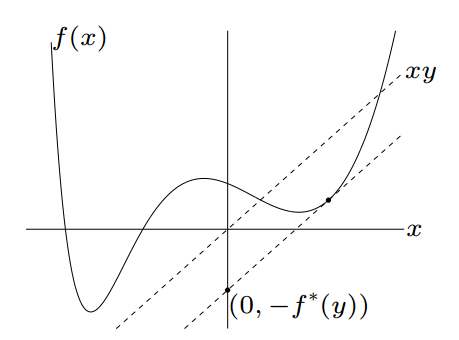
\includegraphics[width=0.4\linewidth]{fig/conjugate.PNG}
	\end{figure}
\end{definition}
由于$f^\star(\vx)$为一系列$\vy$的凸函数的逐点上确界,故$f^\star$为凸函数

\begin{example}
	一些共轭函数的例子如下
	\begin{itemize}
		\item 仿射函数:$f(x)=ax+b$,显然当斜率为$a$时(即平行),共轭函数才有界,故共轭函数定义域为单点集$\{a\}$,且$f^\star(a)=-b$
		\item 最大熵函数:$f(\vx)=\sum_{i=1}^nx_i\log x_i$
		\begin{analysis}
			按照定义进行拆分计算即可
			\[\begin{aligned}
				f^\star(\vy)&=\sup_\vx\sum_{i=1}^n x_i\log x_i\\
				&=\sum_{i=1}^n\sup_{x_i}\lrp{y_i x_i-x_i\log x_i}\qquad\mbox{求导可得}\\
				&=\sum_{i=1}^n\ee^{y_i-1}
			\end{aligned}\]
		\end{analysis}
	\end{itemize}
\end{example}

\subsection{拟凸函数}
\begin{definition}[$\alpha$次水平集($\alpha$-sub level set)]
$f:\rn\mapsto\rr$,$C_\alpha=\{\vx\in\dom f\mid f(\vx)\leq\alpha\}$
\end{definition}
\begin{definition}[拟凸函数(quasi-convex)]
所有$\alpha$次水平集为凸集$\iff$$f$为拟凸函数
\end{definition}
拟凸函数有很好的性质$\to$单模态/单峰函数
\begin{figure}[H]
	\centering
	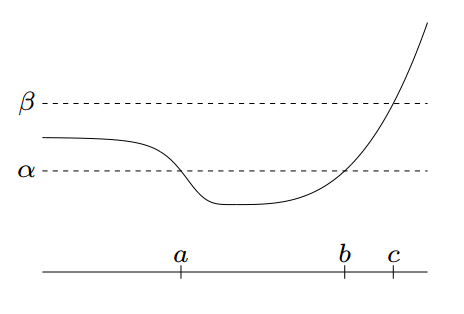
\includegraphics[width=0.4\linewidth]{fig/quasiconvex.PNG}
\end{figure}

\begin{theorem}
	可微拟凸函数判定条件
	\begin{itemize}
		\item 一阶条件:$\dom f$为凸集,且
		\[\forall \vx,\vy\in\dom f:\;f(\vy)\leq f(\vx)\implies\nabla f(\vx)^\T(\vy-\vx)\leq 0\]
		当$\nabla f(\vx)\ne 0$时,即$\nabla f(\vx)$在$\vx$处定义了水平集$\{\vy\mid f(\vy)\leq f(\vx)\}$的支撑超平面
		\begin{figure}[H]
			\centering
			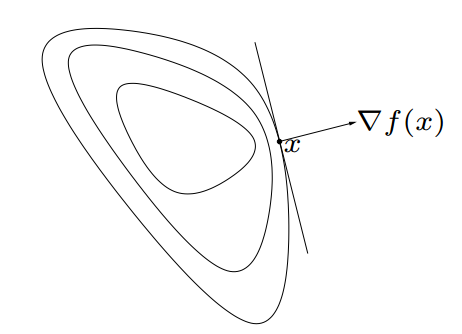
\includegraphics[width=0.4\linewidth]{fig/support-plane.PNG}
		\end{figure}
		\begin{analysis}
			同样考虑一维的情况,然后通过高维定义进行映射
		\end{analysis}
		\item 二阶条件:
		\[\forall \vx\in\dom f,\vy\in\rn:\;\vy^\T\nabla f(\vx)=0\implies \vy^\T\nabla^2f(\vx)\vy\geq 0\]
	\end{itemize}
\end{theorem}

\begin{example}[(拟)凸函数的判定]
	如下图,水平集显然凸(线段都在水平集内),故为拟凸函数,但对于直线\uppercase\expandafter{\romannumeral2},水平集间距离并不是越来越密,故不是凸函数
	\begin{figure}[H]
		\centering
		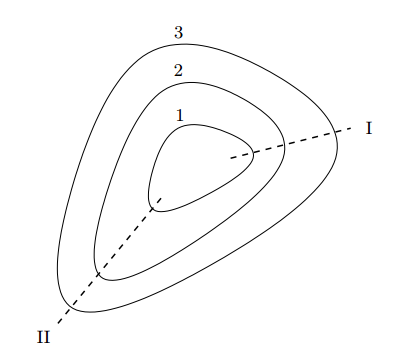
\includegraphics[width=0.35\linewidth]{fig/example-convex-function.PNG}
	\end{figure}
\end{example}

凸函数、拟凸函数与凸集联系
\begin{itemize}
	\item 凸函数定义域为凸集,凸函数一定是拟凸函数
	\item 凸函数的次水平集为凸集,次水平集为凸集的为拟凸函数
\end{itemize}
% !TEX root = main.tex

\section{凸优化问题}
\subsection{标准型}
\label{sub:convex_opt_def}
广义定义:极小化凸函数,约束为凸集
\[\begin{aligned}
& \text{minimize}& f_0(\vx)& &\\
& \text{subject to}& f_i(\vx)&\leq 0 &\quad i&=1,\ldots,m\\
&  & h_j(\vx)&=0 &\quad j&=1,\ldots,p
\end{aligned}\]
\begin{itemize}
	\item 优化变量$\vx\in\rn$
	\item 目标/损失函数$f_0:\rn\mapsto \rr$
	\item 不等式约束函数$f_i:\rn\mapsto \rr$
	\item 等式约束函数$h_j:\rn\mapsto\rr$
	\item 定义域$\sD=\bigcap_{i=0}^m\dom f_i\cap\bigcap_{i=1}^p\dom h_i$(注意不一定可行)
	\item 可行解$\sX=\{\vz\mid f_i(\vz)\leq 0,h_j(\vz)=0,i=1,\ldots,m,j=1,\ldots,p\}$
	\item 最优值(primal) $p^\star=\inf\{f_0(\vx)\mid \vx\in \sX\}$
	\item 最优解$\vx^\star\iff\forall \vz\in\rn,\vz\in\sX:\;f_0(\vz)\geq f_0(\vx^\star)$
	\item 最优解集$\sX^\star=\{\vx^\star\mid f_0(\vx^\star)=p^\star,\vx^\star\in \sS\}$
	\item $\eps$-次优解集$\sX_\eps=\{\vx\mid f_0(\vx)\leq p^\star+\eps, \vx\in \sX\}$
	\item 局部最优$\exists R>0,f_0(\vx)=\inf\{f_0(\vz)\mid \vx\in\sX, \vz\in\sX,\|\vx-\vz\|\leq R\}$,即邻域内下确界
	\item 局部最优解集$\vx_{local}=\{\vx\mid\vx\text{为局部最优}\}$
\end{itemize}

狭义定义:$f_i(\vx),i=0,1,\ldots$为凸函数,$h_i(\vx)$为仿射函数
\begin{example}
	将问题变换为标准型
\begin{mini*}
	{}{f_0(x)=x_1^2+x_2^2}{}{}
	\addConstraint{f_1(x)}{=\frac{x_1}{1+x_2^2}\leq 0}{\implies x_1\leq 0}
	\addConstraint{h_1(x)}{=(x_1+x_2)^2=0}{\implies x_1+x_2=0}
\end{mini*}
\end{example}

% 3.19
\begin{theorem}
凸问题局部最优等价于全局最优
\end{theorem}
\begin{analysis}
若$\vx$为局部最优
\[\exists R>0:\;f_0(\vx)=\inf\{f_0(\vz)\mid \vz\in\sX,\vx\in\sX,\|\vx-\vz\|_2\leq R\}\]
反证法,设$\vx$不是全局最优,$\vy$为全局最优,即$f_0(\vx)>f_0(\vy)$\\
取$\vz=(1-\theta)\vx+ \theta\vy$为$\vx,\vy$连线上一点,令$\theta=\frac{R}{2\|\vy-\vx\|_2}$,使$\vz$能够落在$\vx$的邻域内
\[\|\vz-\vx\|_2=(1-\theta)\norm{\vy-\vx}=\frac{R}{2}\]
由$\|\vz-\vx\|_2\leq R\implies f_0(\vx)\leq f_0(\vz)$,又结合$f_0(\vx)>f_0(\vy)$,有
\[f_0(\vz)\leq\theta f_0(\vx)+(1-\theta)f_0(\vy)<\theta f_0(\vz)+(1-\theta)f_0(\vz)=f_0(\vz)\]
左边第一个不等号由凸函数定义,第二个不等号由推导出的条件,故矛盾
\end{analysis}

\begin{theorem}
对于可微凸目标函数$f_0(\vx)$,最优解满足以下条件
\begin{itemize}
	\item 无约束问题$\min f_0(\vx)$,$\vx^\star$为最优解,当且仅当$\vx^\star\in\sX$,且
	\[\nabla f_0(\vx^\star)=0\]
	\begin{analysis}
	由凸函数的性质
	\[\forall \vx,\vy:\;f_0(\vy)\geq f_0(\vx)+\lrang{\nabla f_0(\vx),\vy-\vx}\]
	进而
	\[f_0(\vy)\geq f_0(\vx^\star)+\lrang{\nabla f_0(\vx^\star),\vy-\vx}=f_0(\vx^\star)\]
	\end{analysis}
	\item 有约束问题$\min f_0(\vx),\,s.t.\,\vx\in\sX$,$\vx^\star$为最优解,当且仅当$\vx^\star\in\sX$,且
	\[\forall \vy\in \sX:\lrang{\nabla f_0(\vx^\star),\vy-\vx^\star}\geq 0\]
	相当于$-\nabla f_0(\vx)$在$\vx$上定义了可行解集的支撑超平面
	\begin{figure}[H]
		\centering
		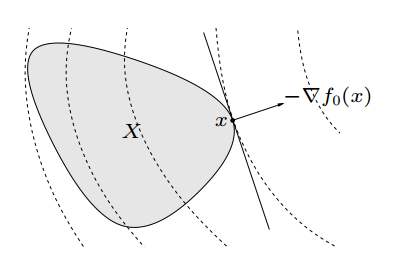
\includegraphics[width=0.4\linewidth]{fig/optimal_criterion_diff.PNG}
	\end{figure}
\end{itemize}
\end{theorem}

\begin{example}[等式约束]
	设$f_0$可微,
	\begin{mini*}
		{}{f_0(\vx)}{}{}
		\addConstraint{A\vx}{=\vb}
	\end{mini*}
\end{example}
\begin{analysis}
设$\vx^\star$为最优解,有$A\vx^\star=\vb$,则最优解需满足
\[\forall \vy, A\vy=\vb:\;\lrang{\nabla f_0(\vx^\star),\vy-\vx^\star}\geq 0\]
对$\vy$进行改写
\[\begin{cases} \vy=\vx^\star+\vv\\A\vv=\vzero\end{cases},\vv\in\opnul A\]
故最优解条件变为
\[\forall \vv\in\opnul A:\;\lrang{\nabla f_0(\vx^\star),\vv}\geq 0\]
那么
\begin{enumerate}
	\item $A$可逆,$\opnul A=\{\vzero\}$
	\item $A$不可逆,$\nabla f_0(\vx^\star)\perp\opnul A$
\end{enumerate}
\end{analysis}

\begin{example}[非负约束]
	设$f_0$可微,
	\begin{mini*}
		{}{f_0(\vx)}{}{}
		\addConstraint{\vx}{\succeq\vzero}
	\end{mini*}
\end{example}
\begin{analysis}
最优性条件为
\[\vx^\star\succeq \vzero,\forall \vy\succeq \vzero:\;\lrang{\nabla f_0(\vx^\star),\vy-\vx^\star}\geq 0
\iff \lrang{\nabla f_0(\vx^\star),\vy}\geq\lrang{\nabla f_0(\vx^\star),\vx^\star}\]
\begin{enumerate}
\item 若$\nabla f_0(\vx^\star)\prec 0$,则存在矛盾($\vy-\vx$全为正),故$\nabla f_0(\vx^\star)\succeq 0$
\item 取$\vy=\vzero$,有
\[0\geq \lrang{\nabla f_0(\vx^\star),\vx^\star}
\implies\sum_{i=1}^n(\nabla f_0(\vx^\star))_ix_i^\star\leq 0
\implies (\nabla f_0(\vx^\star))_i x_i^\star = 0\]
得到\textbf{互补松弛条件},即$\vx$与$\nabla f_0(\vx^\star)$的稀疏模式必须是互补的\\
总结来说,最优性条件为
\[\vx^\star\succeq \vzero\qquad \nabla f_0(\vx^\star)\succeq \vzero\qquad(\nabla f_0(\vx^\star))_i x_i^\star=0,i=1,\ldots,n\]
\end{enumerate}
\end{analysis}

\subsection{线性规划}
当目标函数和约束函数都是仿射时,问题称为线性规划(Linear Programming, LP)
\begin{mini*}
	{}{\vc^\T\vx+d}{}{}
	\addConstraint{G\vx}{\preceq\vh}
	\addConstraint{A\vx}{=\vb}
\end{mini*}
\begin{figure}[H]
	\centering
	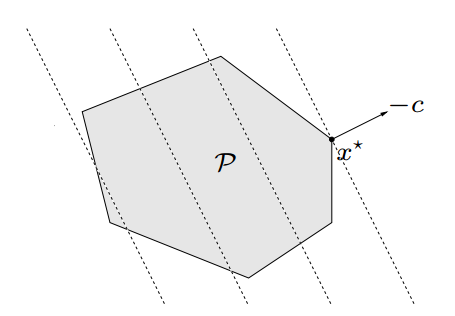
\includegraphics[width=0.35\linewidth]{fig/LP.PNG}
\end{figure}

通过引入松弛变量,对原问题进行变换
\begin{mini*}
	{}{\vc^\T\vx+d}{}{}
	\addConstraint{G\vx+\vs}{=\vh}
	\addConstraint{A\vx}{=\vb}
	\addConstraint{\vs}{\succeq \vzero}
\end{mini*}

进一步,将$\vx$表示为两个非负变量$\vx^+$和$\vx^-$的差,即$\vx=\vx^+ +\vx^-$,得到\textbf{标准型线性规划问题}(不等式都是分量的非负约束)
\begin{mini*}
	{}{\vc^\T\vx^+-\vc^\T\vx^-+d}{}{}
	\addConstraint{G\vx^+-G\vx^-+\vs}{=\vh}
	\addConstraint{A\vx^+-A\vx^-}{=\vb}
	\addConstraint{\vx^+}{\succeq \vzero}
	\addConstraint{\vx^-}{\succeq \vzero}
	\addConstraint{\vs}{\succeq \vzero}
\end{mini*}

\begin{example}[食谱问题]
$m$种营养元素不小于$b_1,\ldots,b_m$,$n$种食物,单位含量$a_{1j},\ldots,a_{mj}$,食物量$x_1,\ldots,x_n$,价格$c_1,\ldots,c_n$
\begin{mini*}
	{}{\sum_{i=1}^n c_jx_j}{}{}
	\addConstraint{\sum_{j=1}^n a_{ij}x_j}{\geq b_i}
	\addConstraint{x_j}{\geq 0}
\end{mini*}
其中$i=1,\ldots,m,j=1,\ldots,n$
\end{example}

% 3.21
\begin{example}[线性分数规划]
	拟凸优化问题
\begin{mini*}
	{}{f_0(\vx)=\frac{\vc^\T \vx+d}{\ve^\T \vx+f}, \dom \vf=\{\vx \mid \ve^\T \vx + f >0 \}}{}{}
	\addConstraint{G\vx}{\preceq \vh}
	\addConstraint{A\vx}{=\vb}
\end{mini*}
等价于
\begin{mini*}
	{\vy,z}{\vc^\T \vy+dz}{}{}
	\addConstraint{G\vy-\vh z}{\preceq 0}
	\addConstraint{A\vy-\vb z}{=0}
	\addConstraint{\ve^\T \vy+fz}{=1}
	\addConstraint{z}{\geq 0}
\end{mini*}
\end{example}
\begin{analysis}
	证明两个问题等价,$P_0$与$P_1$\\
	若$\vx$在$P_0$内可行
	\[\vy=\frac{\vx}{\ve^\T \vx+f},z=\frac{1}{\ve^\T \vx+f}\]
	若$(\vy,z)$在$P_1$中可行
	\[\vx=\frac{\vy}{z}(z\ne 0)\]
	若$z=0$,$x_0$为$P_0$的可行解
	\[\vx=\vx_0+t\vy,t\geq 0\]
	\[\lim_{t\to\infty}\frac{\vc^\T(\vx_0+t\vy)+d}{\ve^\T(\vx_0+t\vy)+f}=\vc^\T \vy\]%考试
	代入看所有条件结论都相同
\end{analysis}

\subsection{二次规划}
当凸优化问题的目标函数为(凸)二次型且约束函数为仿射时,该问题称为二次规划(Quadratic Programming, QP)
\begin{mini*}
	{}{\frac{1}{2}\vx^\T P\vx+\vq^\T\vx+r,\;P\succ 0}{}{}
	\addConstraint{G\vx}{\preceq \vh}
	\addConstraint{A\vx}{=\vb}
\end{mini*}
其中$P\in \mathbb{S}_+^n,G\in\rr^{m\times n},A\in\rr^{p\times n}$

若不等式约束也是(凸)二次型,则成为二次约束二次规划(QCQP)
\begin{mini*}
	{}{\frac{1}{2}\vx^\T P_0\vx+\vq_0^\T \vx+r_0,P_0\succ 0}{}{}
	\addConstraint{\frac{1}{2}\vx^\T P_i\vx+\vq_i^\T \vx+r_i}{\leq 0}{,i=1,\ldots,m}
	\addConstraint{A\vx}{=\vb}
\end{mini*}
其中$P_i\in\mathbb{S}_+^n$

\begin{example}[最小二乘问题的改写]
\begin{mini*}
	{\vx}{\frac{1}{2}\|A\vx-\vb\|_2^2}{}{}
	\addConstraint{A\vx+\ve}{=\vb}
\end{mini*}
\end{example}
\begin{analysis}
一范数规范化最小二乘
\[\min\frac{1}{2}\|A\vx-\vb\|_2^2+\lambda\|\vx\|_1\]
本来用零范数,但用一范数拟合,改写
\[\|\vx\|_1=\vone^\T\vx^+ + \vone^\T\vx^-\]
Basic Pursuit
\begin{mini*}
	{}{\frac{1}{2}\|A\vx-\vb\|_2^2}{}{}
	\addConstraint{\|\vx\|_1}{\leq\eps_1}
\end{mini*}
原式很难平衡两者,下式只需考虑$\|\vx\|_1$的影响\\
采用岭回归(Ridge):所有$\vx$差距不要太大
\[\min\frac{1}{2}\|A\vx-\vb\|_2^2+\frac{1}{2}\lambda_2\|\vx\|_2^2\]
可得类似的问题改写
\begin{mini*}
	{}{\frac{1}{2}\|A\vx-\vb\|_2^2}{}{}
	\addConstraint{\|\vx\|_2^2}{\leq\eps_2}
\end{mini*}
\end{analysis}

\begin{example}[投资组合问题(portfolio optimization)]
初始价格$x_1,\ldots,x_n$,最终价格$P_1x_1,\ldots,P_nx_n$
\begin{maxi*}
	{}{P_1x_1+\cdots+P_nx_n}{}{}
	\addConstraint{x_1+\cdots+x_n}{=B}
	\addConstraint{x_1,\ldots,x_n}{\geq 0}
\end{maxi*}
\end{example}
\begin{analysis}
$\bar{P}=\E{P}$已知,$\Sigma=\Var{P}$
\begin{mini*}
	{}{\vx^\T\Sigma \vx}{}{}
	\addConstraint{\vp^\T \vx}{\geq r_{\min}}
	\addConstraint{\vone^T\vx}{=1}{,\vx\succeq\vzero}
\end{mini*}
\end{analysis}

二次锥规划问题(SOCP)
\begin{mini*}
	{}{\vf^\T\vx}{}{}
	\addConstraint{\norm{A_i\vx+\vb_i}_2}{\leq \vc_i^\T\vx+\vd_i}
	\addConstraint{F\vx}{=\vg}
\end{mini*}

% 3.26
\subsection{广义不等式约束}
半定规划(semi-definite programming, SDP)为矩阵意义下的线性规划问题:% 通信
$X\in\rr^{n\times n},C\in\rr^{n\times n},A_i\in\rr^{n\times n},b_i\in\rr$
\begin{mini*}
	{}{\optr(CX)}{}{}
	\addConstraint{\optr(A_i X)}{=b_i}{,i=1,\ldots,p}
	\addConstraint{X}{\succeq 0}
\end{mini*}

\begin{example}[谱范数极小化问题]
	矩阵多项式$A(\vx)=A_0+x_1A_1+\cdots+x_nA_n,A_i\in\rr^{p\times q}$
	\[\min_\vx\|A(\vx)\|_2\]
	谱范数代表$A(\vx)$的最大奇异值\footnote{谱范数是诱导范数,F-范数(Frobenias)$\|A(\vx)\|_F$才算是矩阵意义下的2范数}
\end{example}
\begin{analysis}
	这是一个$q\times q$矩阵不等式约束的凸优化问题
	\begin{mini*}
		{x,s}{s}{}{}
		\addConstraint{A^\T (\vx)A(\vx)}{\preceq sI}
	\end{mini*}
\end{analysis}

\begin{example}[最快分布式线性平均]
	图的最速混合Markov链
	\[\vx(t) = P\vx(t-1)\]
	其中$P$为邻接矩阵
	\[P=\bmat{P_{11} & \cdots & P_{1n}\\\vdots & \ddots & \vdots\\P_{n1} & \cdots & P_{nn}},P\vone=\vone\]
	其中$(i,j)\in E$或$i=j$,$P_{ij}\ne 0$;否则$P_{ij}=0$\\
	$P=P^\T,P_{ij}=P_{ji}$,$P_{ij}>0,P\succeq 0, P_{ij}\geq 0$
\end{example}
\begin{analysis}
	只要图是连通图,则一定会收敛\\
	收敛速度与第二大[特征值绝对值]有关
	\[1=\lambda_1\geq\lambda_2\geq \cdots\geq \lambda_n\geq -1\]
	即收敛速度由$\max\{|\lambda_2|,|\lambda_n|\}$决定\\
	\[\min\max\{|\lambda_2|,|\lambda_n|\}\]
	\[\max\{|\lambda_2|,|\lambda_n|\}=\norm{P-\frac{1}{n}\vone\vone^\T}\]
	\begin{mini*}
		{}{t:=\norm{P-\frac{1}{n}\vone\vone^\T}_2}{}{}
		\addConstraint{P\vone}{=\vone}
		\addConstraint{P}{=P^\T}
		\addConstraint{P}{\succeq 0}
		\addConstraint{P_{ij}}{= 0,\quad (i,j)\ne E\land i\ne j}
		\addConstraint{-tI}{\preceq P-\frac{1}{n}\vone\vone^\T\preceq tI}
	\end{mini*}
\end{analysis}

\subsection{多目标优化问题}
帕累托最优解:若有另一解在某个指标上更好,则必有指标更差

帕累托最优值/帕累托最优面:$\min f_{01}$与$\min f_{02}$的交点为理想点(oracle)

若$f_{01}(x),\ldots,f_{0q}(x)$为凸,$\sX$为凸
\begin{mini*}[2]
% variable function label LHS
{}{\lambda_1f_{01}(x)+\cdots+\lambda_qf_{0q}(x),\quad\lambda_1,\ldots,\lambda_q\geq 0}{}{}
\addConstraint{x\in\sX}{}
\end{mini*}
\begin{enumerate}
	\item 能找到一个Pareto最优解
	\item 遍历$\lambda_1,\ldots,\lambda_q$,可找到全部
\end{enumerate}

岭回归的多目标优化表示
\[\begin{cases}
	\min \frac{1}{2}\norm{Ax-b}_2^2\\
	\min \frac{1}{2}\norm{x}_2^2
\end{cases}\]
% !TEX root = main.tex

\section{对偶理论}
拉格朗日函数(Lagrangian function)
\[L(x,\lambda,v)=f_0(x)+\sum_{i=1}^m\lambda_if_i(x)+\sum_{i=1}^pv_ih_i(x),\dom L=D\times \rr^m\times \rr^p\]
拉格朗日乘子(multiplier)
\begin{itemize}
\item 原变量(primal variable):$\lambda=\bmat{\lambda_1 & \cdots & \lambda_m}^\T$
\item 对偶变量(dual variable):$v=\bmat{v_1 & \cdots & v_p}^\T$
\end{itemize}

拉格朗日对偶函数
\[\begin{aligned}
    g(\lambda,v)&=\inf_{x\in\sD} L(x,\lambda,v)\\
    &=\inf_{x\in\sD}\lrp{f_0(x)+\sum_{i=1}^m\lambda_if_i(x)+\sum_{i=1}^pv_ih_i(x)}
\end{aligned}\]
注意遍历域是$\sD=\bigcap_{i=0}^m\dom f_i\cap\bigcap_{i=1}^p\dom h_i$,而不是可行解集$\sX$\\
\begin{itemize}
    \item $g(\lambda,v)$一定是关于$\lambda$和$v$的凹函数(关于$\lambda$和$v$的仿射函数,注意$x$为常数)
    \item $\forall\lambda\geq 0,\forall v,g(\lambda,v)\leq P^\star$\\
    对偶(dual)问题
    \begin{maxi*}
        {}{g(\lambda,v)}{}{}
        \addConstraint{\lambda}{\geq 0}
    \end{maxi*}
    其最优解记为$D^\star$,则$D^\star\leq P^\star$,即给出了原问题的一个最优下界
\end{itemize}

$x^\star$原问题最优解
\[\sum_{i=1}^m\lambda_i f_0(x^\star)+\sum_{i=1}^p v_i h_i(x^\star)\leq 0\]
\[L(x^\star,\lambda,v)=f_0(x^\star)+(\cdots)\leq P^\star\]
\[g(\lambda,v)=\inf_{x\in\sD} L(x,\lambda,v)\leq L(x^\star,\lambda,v)\leq P^\star\]

\begin{example}
\begin{mini*}
    {}{x^\T x}{}{}
    \addConstraint{Ax}{=b}
\end{mini*}
\end{example}
\begin{analysis}
\[L(x,v)=x^\T x+v^\T(Ax-b)\]
\[\begin{aligned}
    g(v)&=\inf_{x\in\sD} L(x,v)\\
    &=\inf_{x\in\sD} x^\T x+v^\T A x-v^\T b\\
    &=(-\frac{A^\T v}{2})^\T(-\frac{A^\T v}{2})+v^\T A(-\frac{A^\T v}{2})-v^\T b\\
    &=-\frac{1}{4}v^\T AA^\T v-b^\T v
\end{aligned}\]
补充求梯度:$2x+A^\T v=0\implies x=-\frac{A^\T v}{2}$

因而得到对偶问题
\[\max_v-\frac{1}{4}v^\T AA^\T v-b^\T v\]
\end{analysis}

\begin{example}
\begin{mini*}
    {}{c^\T x}{}{}
    \addConstraint{Ax}{=b}
    \addConstraint{x}{\geq 0}
\end{mini*}
\end{example}
\begin{analysis}
    注意$\lambda$前面符号,要化为一般形式
    \[L(x,\lambda,v)=c^\T x-\lambda^\T x+v^\T(Ax-b)\]
    \[\begin{aligned}
        g(\lambda,v)&=\inf_x L(x,\lambda,v)\\
        &=\inf_x(c-\lambda+A^\T v)^\T x-v^\T b\\
        &=\begin{cases}-\infty&c-\lambda+A^\T v\ne 0\\-v^\T b&c-\lambda+A^\T v=0\end{cases}
    \end{aligned}\]
    对偶问题,由于要极大,故不考虑负无穷部分
    \begin{maxi*}
        {\lambda,v}{-v^\T b}{}{}
        \addConstraint{c-\lambda+A^\T v}{=0}
        \addConstraint{\lambda}{\geq 0}
    \end{maxi*}
    逆过来求解
    \begin{mini*}
        {}{b^\T v}{}{}
        \addConstraint{A^\T v+c}{\geq 0}
    \end{mini*}
    \[L(v,\lambda)=b^\T v-\lambda^\T(A^\T v+c)\]
    \[\begin{aligned}
        g(\lambda)&=\inf_v L(v,\lambda)\\
        &=\inf(b-A\lambda)^\T v-\lambda^\T c\\
        &=\begin{cases}
            -\lambda^\T c & b-A\lambda =0\\
            -\infty & b-A\lambda\ne 0
        \end{cases}
    \end{aligned}\]
    \begin{maxi*}
        {}{-\lambda^\T c}{}{}
        \addConstraint{b-A\lambda}{=0}
        \addConstraint{\lambda}{\geq 0}
    \end{maxi*}
    对偶的对偶不一定回去,线性规划才满足
\end{analysis}
% 对偶支撑向量机(SVM) 升变量维度,降约束维度

\begin{example}
\begin{mini*}
    {}{x^\T wx}{}{}
    \addConstraint{x_i}{=\pm 1,}{\quad i=1,\ldots,n}
\end{mini*}
\end{example}
\begin{analysis}
    \[L(x,v)=x^\T wx+\sum_{i=1}^n v_i(x_i^2-1)\]
    \[\begin{aligned}
        g(v)&=\inf_x L(x,v)\\
        &=\inf_x x^\T wx+\sum_{i=1}^n v_ix_i^2-\sum_{i=1}^n v_i\\
        &=\inf_x x^\T\lrp{w+\opdiag v}x-\vone^\T v
        &=\begin{cases}-\vone^\T v & w+\opdiag(v)\succeq 0\\-\infty&\text{otherwise}\end{cases}
    \end{aligned}\]
    补充求梯度:$2(w+\opdiag(v))x=0$
    \begin{maxi*}
        {v}{-\vone^\T v}{}{}
        \addConstraint{w+\opdiag(v)}{\succeq 0}
    \end{maxi*}
\end{analysis}

\begin{definition}[函数的共轭]
    $f:\rn\mapsto\rr,f^\star(y)=\sup_{x\in\dom f}(y^\T x-f(x))$,
    几何意义即到不同斜率直线的距离最大值
\end{definition}
\begin{mini*}
    {}{f_0(x)}{}{}
    \addConstraint{Ax}{\leq b}
    \addConstraint{cx}{=d}
\end{mini*}
\[\begin{aligned}
    L(x,\lambda,v)&=f_0(x)+\lambda^\T(Ax-b)+v^\T(cx-d)\\
    &=f_0(x)+(A^\T\lambda+c^\T v)^\T x-\lambda^\T b-v^\T d\\
    g(\lambda,v)&=\inf_x f_0(x)+(A^\T\lambda+c^\T v)^\T x-\lambda^\T b-v^\T d\\
    &=-\sup_x-(A^\T\lambda+c^\T v)^\T x-f_0\\
    &=-f_0^\star(-(A^\T\lambda+c^\T v))-\lambda^\T b-v^\T d
\end{aligned}\]

对偶间隙(duality gap):$p^\star-d^\star\geq 0$
\begin{itemize}
    \item 弱对偶:严格大于0
    \item 强对偶:对偶间隙为0
\end{itemize}

\begin{enumerate}
    \item 对于非凸问题,\textbf{通常}$p^\star\ne d^\star$
    \item 对于凸问题,若slater条件满足,$p^\star=d^\star$
\end{enumerate}

\begin{definition}[相对内点(relative interior)]
    \[\mathop{relint} D=\{x\in D\mid B(x,r)\cap\opaff D\subset v,\exists r>0\}\]
\end{definition}

\begin{theorem}[Slater条件]
\begin{mini*}
    {}{f_0(x)}{}{}
    \addConstraint{f_i(x)}{\leq 0}{,\quad i=1,\ldots,m}
    \addConstraint{Ax}{=b}
\end{mini*}
$\exists x\in\mathop{relint} D$使得$f_i(x)<0,i=1,\ldots,m,Ax=b$
\end{theorem}
\begin{example}
    二次规划(QP)
    \begin{mini*}
        {}{x^\T x}{}{}
        \addConstraint{Ax}{=b}
    \end{mini*}
    Slater条件$\{x\mid Ax=b\}$非空
\end{example}
\begin{example}
    二次约束二次规划(QCQP)
    \begin{mini*}
        {}{\frac{1}{2}x^\T P_0 x+q_0^\T+r_0}{}{}
        \addConstraint{\frac{1}{2}x^\T P_i x+q_i^\T x+r_i}{\leq 0}{,\quad i=1,\ldots,m}
    \end{mini*}
    $P_0,\ldots,P_i$半正定
\end{example}

凸问题+Slater条件$\implies p^\star=d^\star$,但有可能不满足Slater条件也依然强对偶
\begin{example}
\begin{mini*}
    {}{x,x\in\rr}{}{}
    \addConstraint{x}{leq 0}
    \addConstraint{-x}{\leq 0}
\end{mini*}
\end{example}
\begin{analysis}
    \[L(x,\lambda_1,\lambda_2)=x+\lambda_1 x-\lambda_2 x=(1+\lambda_1-\lambda_2)x\]
\[g(\lambda_1,\lambda_2)=\inf_{x\in\rr}(1+\lambda_1-\lambda_2)x=
\begin{cases}0& 1+\lambda_1-\lambda_2=0\\ -\infty &\text{otherwise}\end{cases}\]
    \begin{maxi*}
        {\lambda_1,\lambda_2}{0}{}{}
        \addConstraint{1+\lambda_1-\lambda_2}{=0}
    \end{maxi*}
\[\implies p^\star=d^\star=0\]
\end{analysis}

置信域问题
\begin{mini*}
    {}{x^\T Ax+b^\T x}{}{}
    \addConstraint{x^\T x}{\leq 1}
    \addConstraint{A}{\nsucceq 0}
\end{mini*}
依然可以得到$p^\star=d^\star$

几何解释
\begin{mini*}
    {}{f_0(x)}{}{}
    \addConstraint{f_i(x)}{\leq 0}{,\quad i=1,\ldots,m}
\end{mini*}

\[G=\{(f_1(x),f_0(x))\mid x\in\sD\}\]
\[g(\lambda)=\inf\{t+\lambda u\mid(u,t)\in G\}\]
\[L(x,\lambda)=f_0(x)+\lambda f_1(x)\]
\[g(\lambda)=\inf_{x\in\sD}\{f_0(x)+\lambda f_1(x)\}\]

\[p^\star=\inf\{t\mid(u,t)\in G,u\leq 0\}\]
\[\lambda\geq 0,\max g(\lambda)\]

注意问题必须要有可行解

经济学解释:满足原材料约束下,利润最多
价格$\lambda_i\geq 0$
\[g(\lambda)=\inf_x f_(x)+\lambda_1 f_1(x)+\cdots+\lambda_m f_m(x)=\inf_x L(x,\lambda)\]
则$g(\lambda)$为对偶函数,市场$p^\star$损失最小($g(\lambda)\leq p^\star$)
\[d^\star=\sup_{lambda\geq 0}g(\lambda)\]
市场平衡点,均衡市场$p^\star=d^\star$,最优/影子价格$\lambda^\star$

多目标优化解释
\[\begin{cases}
    \min f_0(x) & 1\\
    \min f_1(x) & \lambda_1\\
    \vdots & \vdots\\
    \min f_m(x) & \lambda_m
\end{cases}\]
\[\min_x f_0(x)+\lambda_1 f_1(x)+\cdots+\lambda_m f_m(x)\]

鞍点(saddle point)解释
\[f(w,z),w\in S_w,z\in S_z\]
极小极大不等式
\[\sup_{z\in S_z}\inf_{w\in S_w} f(wz)\leq \inf_{w\in S_w}\sup_{z\in S_z}f(w,z)\]
若有$(\tilde{w},\tilde{z})$使得
\[\begin{aligned}
    (\tilde{w},\tilde{z})&=\arg\max_{z\in S_z}\min_{w\in S_w} f(w,z)
    (\tilde{w},\tilde{z})&=\arg\min_{w\in S_w}\max_{z\in S_z} f(w,z)
\end{aligned}\]
则$(\tilde{w},\tilde{z})$为鞍点

有下面不等式成立
\[f((\tilde{w},z))\leq f(\tilde{w},\tilde{z})\leq f(w,\tilde{z}),\forall z\in S_z,w\in S_w\]
即从一个方向望过去是最小,从另一个方向望过去是最大

\[\begin{aligned}
    &L(x,\lambda)&=f_0(x)+\sum_{i=1}^m\lambda_i f_i(x)\\
    \implies&\sup_{\lambda\geq 0}L(x,\lambda)&=\sup_{\lambda\geq 0}\{f_0(x)+\sum_{i=1}^m\lambda_if_i(x)\}\\
    &&=\begin{cases}f_0(x)&f_i(x)\leq 0,i=1,\ldots,m\\+\infty&\text{otherwise}\end{cases}\\
    \implies& p^\star&=\inf_x\{f_0(x)\mid f_i(x)\leq 0,i=1,\ldots,m\}=\inf_x\sup_{\lambda\geq 0}L(x,\lambda)
\end{aligned}\]
\[d^\star=\sup_{\lambda\geq 0}g(\lambda)=\sup_{\lambda\geq 0}\inf_x L(x,\lambda)\implies p^\star\geq d^\star\]

如果$L(x,\lambda)$有鞍点,则必有$p^\star=d^\star$

鞍点在无约束优化问题中是很糟糕的点(所有方向上梯度为0),但是有约束优化问题则是非常好的点

若$(\tilde{x},\tilde{\lambda})$为$L(x,\lambda)$鞍点$\iff p^\star=d^\star$且$\tilde{x},\tilde{\lambda}$为原对偶问题最优解
$\implies$若为鞍点,$p^\star=d^\star$
\[\sup_{\lambda\geq 0}\inf_x L(x,\lambda)=\inf_x\sup_{\lambda\geq 0}L(x,\lambda)\]
已知$(\tilde{x},\tilde{\lambda})$为左边最优
\[\begin{aligned}
    \tilde{\lambda}&=\arg\max_{\lambda\geq 0}\inf_x L(x,\lambda)\\
    \tilde{x}&=\arg\inf_x\sup_{\lambda\geq 0}L(x,\lambda)
\end{aligned}\]
则$\tilde{\lambda}$对偶最优,$\tilde{x}$为原问题最优

% 4.4
\begin{mini*}
    {}{f_0(x)}{}{}
    \addConstraint{f_i(x)}{\leq 0}{,\quad i=1,\ldots,m}
\end{mini*}
\begin{theorem}
    $(\tilde{x},\tilde{\lambda})$为拉格朗日函数鞍点$\iff p^\star=d^\star$,且$(\tilde{x},\tilde{\lambda})$为原对偶的最优解
\end{theorem}
\begin{analysis}
    右推左,$(\tilde{x},\tilde{\lambda})$原对偶可行
    \[f_i(\tilde{x})\leq 0,i=1,\ldots,m,\tilde{\lambda}\geq 0\]
    因$p^\star=d^\star$,有
    \[\begin{aligned}
        f_0(\tilde{x})&=g(\tilde{\lambda})\\
        &=\inf_x\{f_0(x)+\sum_{i=1}^m\tilde{\lambda}_i f_i(x)\}\\
        \leq & f_0(\tilde{x})+\sum_{i=1}^m\tilde{\lambda}_i f_i(\tilde{x})\\
        \leq & f_0(\tilde{x})
    \end{aligned}\]
    进而不等号都得为等号
    \begin{enumerate}
        \item $\inf_x L(x,\tilde{\lambda})=L(\tilde{x},\tilde{\lambda})$
        \item $f_0(\tilde{x})=\sup_{\lambda\geq 0}\{f_0(\tilde{x})+\sum_{i=1}^m\lambda_i f_i(\tilde{x})\}=\sup_{\lambda\geq 0}L(\tilde{x},\lambda)$
    \end{enumerate}
    \[\implies L(\tilde{x},\tilde{\lambda})=\sup_{\lambda\geq 0}L(\tilde{x},\lambda)\]
    \[\implies (\tilde{x},\tilde{\lambda})\text{是}L(x,\lambda)\text{的鞍点}\]
\end{analysis}

一般优化问题的对偶理论
\begin{mini*}
    {}{f_0(x)}{}{}
    \addConstraint{f_i(x)}{\leq 0}{,\quad i=1,\ldots,m}
    \addConstraint{h_i(x)}{=0}{,\quad i=1,\ldots,p}
\end{mini*}
不一定是凸问题,但$p^\star=d^\star$,最优解满足什么条件?

对偶问题
\begin{maxi*}
    {}{g(\lambda,v)}{}{}
    \addConstraint{\lambda}{\geq 0}
\end{maxi*}
\begin{analysis}
    设$(x^\star,\lambda^\star,v^\star)$为原对偶最优解,则$(x^\star,\lambda^\star,v^\star)$为原对偶可行解
    \[f_i(x^\star)\leq 0,i=1,\ldots,m,\quad h_i(x^\star)=0,i=1,\ldots,p,\quad\lambda^\star\geq 0\]
    \[\begin{aligned}
        p^\star=d^\star\implies f_0(x^\star)&=g(\lambda^\star,v^\star)\\
        &=\inf_x\{f_0(x)+\sum_{i=1}^m\lambda_i^\star f_i(x)+\sum_{i=1}^pv_i^\star h_i(x)\}\\
        &\leq f_0(x^\star)+\sum_{i=1}^m\lambda_i^\star f_i(x^\star)+\sum_{i=1}^pv_i^\star h_i(x^\star)\\
        &\leq f_0(x^\star)
    \end{aligned}\]
    同上理,不等号全取等
    \begin{enumerate}
        \item $\lambda_i^\star f_i(x^\star)=0,\forall i=1,\ldots,m$
        \item $x^\star=\arg\min_x L(x,\lambda^\star,v^\star)$
    \end{enumerate}
    若$f_0,f_i,h_i$均可微,则必要条件为
    \[\pd{L(x,\lambda^\star,v^\star)}{x}\Big|_{x=x^\star}=0\]
\end{analysis}
可微优化问题的KKT(Karush-Kuhn-Tucker)条件
\begin{itemize}
    \item $f_i(x^\star)\leq 0,i=1,\ldots,m$ primal feasibility
    \item $h_i(x^\star)=0,i=1,\ldots,p$ primal feasibility
    \item $\lambda^\star\geq 0$ dual feasibility
    \item $\lambda_i^\star f_i(x^\star)=0, i=1,\ldots,m$ complementarity slackness(对偶互斥条件)
    \item $\pd{L(x,\lambda^\star,v^\star)}{x}\Big|_{x=x^\star}=0$ stablity
\end{itemize}

\begin{theorem}
若原问题为凸,则KKT条件为\textbf{充要条件}
\end{theorem}
\begin{analysis}
    必要性已证,证明充分性\\
    若$(\tilde{x},\tilde{\lambda},\tilde{v})$满足KKT条件$\implies(\tilde{x},\tilde{\lambda},\tilde{v})$最优
    $\tilde{x}$为原问题可行解,$(\tilde{\lambda},\tilde{v})$为对偶问题可行解\\
    证明思路:$g(\tilde{\lambda},\tilde{v})=f_0(\tilde{x})$\\
    $L(x,\tilde{\lambda},\tilde{v})$为$x$的凸函数,则$\tilde{x}$使$L(x,\tilde{\lambda},\tilde{v})$最小
    \[\begin{aligned}
        g(\tilde{\lambda},\tilde{v})&=\inf_x L(x,\tilde{\lambda},\tilde{v})\\
        &=L(\tilde{x},\tilde{\lambda},\tilde{v})\\
        &=f_0(\tilde{x})+\sum_{i=1}^m\tilde{\lambda}_if_i(\tilde{x})+\sum_{i=1}^p\tilde{v_i}h_i(\tilde{x})\\
        &=f_0(\tilde{x})
    \end{aligned}\]
\end{analysis}

\begin{example}[Waterfilling算法]
    共$n$个信道(channel)
    \begin{center}
        \begin{tikzcd}
            \text{source}\arrow{r} & \text{destination}\arrow{l}
        \end{tikzcd}
    \end{center}
    \begin{mini*}
        {}{-\sum_{i=1}^n\log(\alpha_i+x_i)}{}{}
        \addConstraint{x}{\geq 0}
        \addConstraint{\vone^\T}{=1}
    \end{mini*}
\end{example}
\begin{analysis}
    KKT条件
    \begin{itemize}
        \item $x^\star\geq 0$
        \item $\vone^\T x^\star=1$
        \item $\lambda^\star\geq 0$
        \item $x_i^\star\lambda_i^\star=0,\forall i$
    \end{itemize}
\[\begin{aligned}
    L(x,\lambda,v)=-\sum_{i=1}^n\log(\alpha_i+x_i)-\lambda^\T x+v(\vone^\T x-1)
\end{aligned}\]
\[\lrp{\pd{L(x,\lambda,v)}{x}}_i=-\frac{1}{\alpha_i+x_i}-\lambda_i+v\]
\[-\frac{1}{\alpha_i+x_i^\star}-\lambda_i^\star+v^\star=0,\forall i\]
\[\implies v^\star\frac{1}{\alpha_i+x_i^\star},i=1,\ldots,n\]
\[x_i^\star\lrp{v^\star-\frac{1}{\alpha_i+x_i^\star}}=0,i=1,\ldots,n\]
若$v^\star>\frac{1}{\alpha_i}\implies x_i^\star=0$\\
若$v^\star<\frac{1}{\alpha_i}$
\[\frac{1}{\alpha_i}>v^\star\geq\frac{1}{\alpha_i+x_i^\star}\]
进而
\[\begin{aligned}
    x_i^\star&>0\\
    v^\star&=\frac{1}{\alpha_i+x_i^\star}\\
    x_i^\star&=\frac{1}{v^\star}-\alpha_i
\end{aligned}\]
\[\implies x_i^\star=\max\{0,\frac{1}{v^\star}-\alpha_i\}\]
结合$\sum_i x_i^\star=1$,即注水算法
\end{analysis}

Motivation:误差,调整参数测灵敏度
\begin{mini*}
    {}{f_0(x)}{}{}
    \addConstraint{f(x)}{\leq u_i}{,\quad i=1,\ldots,m}
    \addConstraint{h_i(x)}{= w_i}{,\quad i=1,\ldots,p}
\end{mini*}
新问题的最优解记为$p^\star(\vu,\vw)$

性质:若原始问题为凸,则$p^\star(\vu,\vw)$是$(u,w)$的凸函数

布尔线性规划问题做松弛(relaxation)
\[x_i\in\{0,1\}\implies 1\geq x_i\geq 0\]
% !TEX root = main.tex

\section{优化算法}
\subsection{简介}
\begin{mini*}
    {}{f_0(x)}{}{}
    \addConstraint{A\vx}{=\vb}
\end{mini*}
罚函数法
\[\min f_0(x)+\frac{\lambda}{2}\norm{A\vx-\vb}_2^2\]
\[\tilde{x}=\arg\min_x F\]
\[\nabla f_0(\tilde{\lambda})+\lambda A^\T(A\tilde{\vx}-\vb)=0\]
\[\begin{aligned}
    L(x,v)&=f_0(x)+v^\T(A\vx-\vb)\\
    \implies g(v)&=\inf_x f_0(x)+v^\T(A\vx-\vb)\\
    v&=\lambda(A\tilde{\vx}-\vb)\\
    \implies & g(\lambda(A\tilde{x}-\vb)=\inf_x f_0(x)+\lambda(A\tilde{x}-b)^\T(A\vx-\vb)
\end{aligned}\]
\[\nabla f_0(x)+\lambda A^\T(A\tilde{x}-\vb)=0\]

\begin{mini*}
    {}{f_0(x)}{}{}
    \addConstraint{A\vx}{\geq\vb}
\end{mini*}
log-barrier
\[\min f_0(x)+\sum_{i=1}^m u_i\log(a_i^\T \vx-b_i)\]


$\min f_0(x)$可微,凸,无约束
\begin{enumerate}
    \item 所有算法都是迭代的
    \[\iter{x}{k+1}=\iter{x}{k}+\iter{\alpha}{k}\iter{d}{k}\]
    $\alpha\geq 0$为步长,$d$为方向,所有算法本质上都是选择方向与步长的问题
    \item 如何选择步长$\iter{\alpha}{k}$
    \[\begin{cases}
    \text{确定步长} & \begin{cases}\text{固定步长}\\\text{变化步长(递减步长)}\end{cases}\\
    \text{搜索步长}
    \end{cases}\]
    最优步长:线搜索问题
    \[\iter{\alpha}{k}=\arg\min_{\alpha\geq 0} f_0(\iter{x}{k}+\alpha\iter{d}{k})\]
    \item 关键问题是选方向
\end{enumerate}
黄金分割法(0.618法)/优选法求解线搜索问题:这样做的采样复杂度很低,之前算过的点很容易被再用!

不精确线搜索(Armijo Rule):一阶泰勒展开
% \begin{algorithm}[H]
%     \begin{algorithmic}[1]
%         \State{$\iter{\alpha}{k}=\alpha_\max$}
%         \If{$f_0(\iter{x}{k}+\iter{\alpha}{k}\iter{d}{k})>f_0(\iter{x}{k}+\mu\iter{\alpha}{k}\lrang{\nabla f_0(\iter{x}{k},\iter{d}{k})})$}
%         \State $\iter{\alpha}{k}\gets\iter{\alpha}{k}\beta,\beta\in(0,1)$
%         \Else
%         \State Stop
%         \EndIf
%     \end{algorithmic}
% \end{algorithm}

实际上没有必要求最优步长,在该方向上的差异并没有太大

\subsection{梯度下降法}
$\iter{d}{k}=-\nabla f_0(\iter{x}{k})$
\begin{itemize}
    \item 能否收敛
    \item 收敛到哪里
    \item 收敛速度
\end{itemize}

假设
\begin{itemize}
    \item[0.] 基本假设:$f$为可微的凸函数,
    \[x^\star=\arg\min_x f_0(x)\]
    存在且有限,$f_0(x^\star)$有限
    \item[1.] Lipschitz连续梯度
    \[\exists L>0,\norm{\nabla f_0(x)-\nabla f_0(y)}\leq L\norm{x-y},\forall x,y\]
    \item[2.] 强凸性(strong convexity)
    \[\exists\mu>0:\;f_0(y)\geq f_0(x)+\lrang{\nabla f_0(x),y-x}+\frac{\mu}{2}\norm{x-y}_2^2,\forall x,y\]
\end{itemize}
% !TEX root = main.tex

\section{大数据中的优化问题与算法}
\subsection{并行优化}
\begin{center}
    \begin{tikzcd}
        & \text{master }g(\vx)\arrow{dl}\arrow{d}\arrow{dr} & \\
        \text{worker1 }f_1(\vx) & \text{worker2 }f_2(\vx) & \text{worker3 }f_3(\vx)
    \end{tikzcd}
\end{center}
\[\min_x\; g(\vx)+\sum_{i=1}^N f_i(\vx)\]

针对LASSO问题,每个人都有一个样本$(A_i,\vb_i)$,最小化样本之和,以及正则化项
\[\begin{cases}
    (A_1,\vb_1)\implies\frac{1}{2}\norm{A_1 \vx-\vb_1}_2^2\\
    \vdots\\
    (A_n,\vb_n)\implies\frac{1}{2}\norm{A_N \vx-\vb_N}_2^2\\
    g(\vx)=v\norm{\vx}_1
\end{cases}\]
原问题即为
\[\min_x\; v\norm{\vx}_1+\frac{c}{2}\norm{\bmat{A_1 & \cdots & A_N}\vx-\bmat{\vb_1 & \cdots & \vb_N}}_2^2\]

\subsubsection{并行梯度下降法}
\[\begin{cases}
    \iter{\vx}{k+\frac{1}{2}}=\iter{\vx}{k}-\alpha\sum_{i=1}^N\nabla f_i(\iter{\vx}{k})\\
    \iter{\vx}{k+1}=\arg\min g(\vx)+\frac{1}{2\alpha}\norm{\vx-\iter{\vx}{k+\frac{1}{2}}}_2^2
\end{cases}\]
计算简单,只需求梯度,但所有梯度类问题都依赖于条件数。通信开销大。

\subsubsection{对偶分解法}
\begin{mini*}
    {}{\sum_{i=1}^N f_i(\vx_i)+g(\vz)}{}{}
    \addConstraint{\vx_i}{=\vz,\forall i}
\end{mini*}
\[L(\vx,\vz,\vv)=\sum_{i=1}^N f_i(\vx_i)+g(\vz)+\sum_{i=1}^N\lrang{\vv_i,\vx_i \vz}\]
\[(\iter{\vx}{k+1},\iter{\vz}{k+1})=\arg\min_{\vx,\vz}L(\vx,\vz,\iter{v}{k})\]
\[\implies\begin{cases}
    \iter{\vx_i}{k+1}=\arg\min_{\vx_i} f_i(\vx_i)+\lrang{\iter{\vv_i}{k},\vx_i}\\
    \iter{\vz}{k+1}=\arg\min_{\vz_i} g(\vz)-\sum_{i=1}^N\lrang{\iter{\vv_i}{k},\vz}\\
    \iter{\vv_i}{k+1}=\iter{\vv_i}{k}+\alpha\lrang{\iter{\vx_i}{k+1},\iter{\vz}{k+1}}
\end{cases}\]
不依赖于条件数,但每一步都需要求解一个最优解,不一定好求。通信开销小,但拉格朗日类方法收敛性差。

\subsubsection{增广拉格朗日函数}
\[\sum_{i=1}^nf_i(\vx_i)+g(\vz)+\sum_{i=1}^n\lrang{\lambda_i,\vx-\vz}+\frac{c}{2}\sum_{i=1}^n\norm{\vx_i-\vz}^2\]
正则项会产生$\vx_i$和$\vz$的交叉项,不好处理

注意到$\vx_i$之间是没有依赖的,故采用交替方向乘子法,加了增广项,可用固定步长达到最优解
\[\begin{cases}
    \iter{\vx_i}{k+1}&=\arg\min f_0(\vx_i)+\lrang{\iter{\lambda_i}{k},\vx_i}+\frac{c}{2}\norm{\vx_i-\iter{\vz}{k}}^2\\
    \iter{\vz}{k+1}&=\arg\min g(\vz)-\lrang{\sum_{i=1}^n\iter{\lambda_i}{k},\vz}+\frac{c}{2}\sum_{i=1}^n\norm{\iter{\vx_i}{k+1}-\vz}^2\\
    \iter{\lambda}{k+1}&=\iter{\lambda}{k}+c(\iter{\vx_i}{k+1}-\iter{\vz}{k+1})
\end{cases}\]
每次要多传一倍的变量,以通信量开销换性能提升

\subsection{无中心分布式优化}
\par 考虑无向图
\begin{center}
    \begin{tikzcd}
        & o\arrow{r}\arrow{ld}\arrow{rd} & o\arrow{d}\\
        o\arrow{rd} & & o\arrow{ld}\arrow{d}\\
        & o\arrow{uu} & o\arrow{l}
    \end{tikzcd}
\end{center}
每个结点自己优化,协同决策
\[\min\sum_{i=1}^n f_i(\vx)\]
梯度下降法,但由于去中心,$\iter{\vx}{k}$无处摆放
\[\iter{\vx}{k+1}=\iter{\vx}{k}-\iter{\alpha}{k}\sum_{i=1}^n\nabla f_i(\iter{\vx}{k})\]
那就每一个点分配一个本地变量$\vx_i$,对邻居的更新做一个加权平均
\[\iter{\vx}{k+1}=\sum_{i=1}^n\omega_{ij}\iter{\vx_j}{k}-\iter{\alpha}{k}\sum_{i=1}^n\omega_{ij}\nabla f_j(\iter{\vx_j}{k})\]
其中
\[\begin{cases}
    \omega_{ij}\ne 0 & (i,j)\in E, i=j\\
    \omega_{ij}=0 & \text{otherwise}
\end{cases}\]
\[W=\bmat{\omega_{ij}},W=W^\T,W\vone=\vone\]

在不可信的系统里面,存在个人隐私等信息,故更激进些,采用自己的梯度进行更新(在本地进行梯度下降),在无人机系统中非常常见
\[\iter{\vx_i}{k+1}=\sum_{i=1}\omega_{ij}\iter{\vx_j}{k}-\iter{\alpha}{k}\nabla f_i(\iter{\vx_i}{k})\]
非常糟糕的算法,如果采用固定步长,则找不到最优解
\begin{analysis}
反证法,假设$\iter{\vx_i}{k}\to \vx^\star$,将$\vx^\star$代入
\[\vx^\star=\sum_{j=1}^n\omega_{ij}\vx^\star-\alpha\nabla f_i(\vx^\star)\iff \nabla f_i(\vx^\star)=0\]
但原问题最优解
\[\sum_{i=1}^n\nabla f_i(\vx^\star)=0\]
与上面的式子不等价
\end{analysis}

改成有约束优化的形式
\begin{mini*}
    {}{\sum_{i=1}^n f_i(\vx_i)}{}{}
    \addConstraint{\vx_1=\vx_2=\cdots=\vx_n}
\end{mini*}
写出拉格朗日函数,对偶分解法
\[\sum_{i=1}^nf_i(\vx_i)+\sum_{(i,j)\in E}\lrang{\vlambda_{ij},\vx_i-\vx_j}\]
别人的东西都在对偶变量中体现,求同存异
\[\begin{cases}
    \iter{\vx_i}{k+1}=\arg\min f_i(\vx_i)+\sum_{(i,j)\in E}(\iter{\vlambda_{ij}}{k},\vx_i)-\sum_{(j,i)\in E}\lrang{\vlambda_{ij},\vx_i}\\
    \iter{\vlambda_{ij}}{k+1}=\iter{\vlambda_{ij}}{k}+\iter{\alpha}{k}(\iter{\vx_i}{k+1}-\iter{\vx_j}{k+1})-\sum_{(j,i)\in E}\lrang{\iter{\vlambda_{ij}}{k}\vx_i}
\end{cases}\]
依然要采用递减步长,才能保证收敛

\begin{center}
    \begin{tikzcd}
        \vx_i\arrow[bend left]{rr}{\vz_{ij}} & & \vx_j\arrow[bend left]{ll}{\vz_{ji}}
    \end{tikzcd}
\end{center}
\begin{mini*}
    {}{\sum_{i=1}^n f_i(\vx_i)}{}{}
    \addConstraint{\vx_i}{=\vz_{ij},\forall (i,j)\in E}
    \addConstraint{\vx_j}{=\vz_{ji},\forall (i,j)\in E}
\end{mini*}
可分线性约束,进而可以用交替方向乘子法

\[\begin{aligned}
    \sum_{i=1}^nf_i(\vx_i)&+\sum_{(i,j)\in E}\lrp{\lrang{\valpha_{ij},\vx_i-\vz_j}+\lrang{\vbeta_{ij}{k}\vx_j-\vz_{ji}}}\\
    &+\sum_{(i,j)\in E}\frac{c}{2}\lrp{\norm{\vx_i-\vz_{ij}}^2+\norm{\vx_j-\vz_{ij}}^2}
\end{aligned}\]
\[\begin{cases}
    \iter{\vx_i}{k+1}&=\arg\min f_i(\vx_i)+\sum_{(i,j)\in E}\lrang{\iter{\alpha_{ij}{k}},\vx_i}+\sum_{(i,j)\in E}\lrang{\iter{\vbeta_{ji}}{k},\vx_i}\\
    \qquad&+\frac{c}{2}\sum_{(i,j)\in E}\norm{\vx_i-\iter{\vz_j}{k}}^2+\frac{c}{2}\sum_{(i,j)\in E}\norm{\vx_i-\iter{\vz_{ji}}{k}}^2\\
    \iter{\vz_j}{k+1}&=\cdots\\
    \iter{\valpha_{ij}}{k+1}&=\cdots\\
    \iter{\vbeta_{ij}}{k+1}&=\cdots
\end{cases}\]

\subsection{有限和优化}
$n$个样本,每个样本为$f_i(\vx)$
\begin{mini*}
    {\vx}{\frac{1}{n}\sum_{i=1}^nf_i(\vx)}{}{}
\end{mini*}
等价于期望极小化问题
\begin{mini*}
    {\vx}{\E{f_i(\vx,\xi)}}{}{}
\end{mini*}

\[\iter{\vx}{k+1}=\iter{\vx}{k}-\alpha\frac{1}{n}\sum_{i=1}^n\nabla f_i(\iter{\vx}{k})\]
将$k$改为$\iter{i}{k}$,随机梯度下降(Stochastic gradient descent, SGD),取了一个无偏的估计[Bottou, NIPS 2010]
\[\iter{\vx}{k+1}=\iter{\vx}{k}-\iter{\alpha}{k}\nabla f_{\iter{i}{k}}(\iter{\vx}{k})\]
注意这里需要采用变步长,否则无法收敛到最优解
\[\begin{cases}
    \iter{\vx}{k+1}=\iter{\vx}{k}-\iter{\alpha}{k}\nabla f_{\iter{i}{k}}(\iter{\vx}{k})\\
    \vx^\star=\vx^\star-\iter{\alpha}{k}\nabla f_{\iter{i}{k}}(\vx^\star)
\end{cases}\implies\nabla f_{\iter{i}{k}}(\vx^\star)=0\]

若问题强凸,$O(\frac{1}{k})\to O(\frac{1}{k})$;
凸,$O(\frac{1}{\sqrt{k}})\to O(\frac{1}{\sqrt{k}})$

梯度噪声的问题:选的随机梯度与真正的全梯度不同

\subsection{方差消减}
方差消减(Variance Reduction):挑选样本数目增大时,方差会减小
\begin{enumerate}
\item 小批量(mini-batch)
\item SURG、SAG、SAGA
\[\iter{\vx}{k+1}=\iter{\vx}{k}-\frac{\alpha}{n}\sum_{i=1}^n\iter{y_i}{k}\]
对于每一个样本都存储一个梯度值
\[\iter{y_i}{k}=\begin{cases}
    \nabla f_i(\iter{\vx}{k}) & i=\iter{i}{k}\\
    \iter{y_i}{k-1} & i\ne\iter{i}{k}
\end{cases}\]
当时间足够长,每一个里面都存在最优梯度
\[\vx^\star=\vx^\star-\frac{\alpha}{n}\sum_{i=1}^n\nabla f_i(\vx^\star)\]
相当于用空间换时间
\end{enumerate}

\subsection{深度神经网络}
\begin{mini*}
    {}{\sum_{i=1}^S \iter{E}{i}}{}{}
\end{mini*}
其中,
\[\iter{E}{i}=\frac{1}{2}\norm{\iter{\vx_n}{i}-\iter{Y}{i}}^2\]
为损失函数,$\vx_n$为第$n$层的网络输出$f_n(\vx_{n-1},\omega_n)$,与有限和优化问题相同

反向传播算法(Back propagation):自底向上求出$E$相对于$\vx_n$和$w_n$的梯度
\[\begin{cases}
    \pd{\iter{E}{i}}{\iter{\vx_n}{i}}=\iter{\vx_n}{i}-\iter{Y}{i}\\
    \pd{\iter{E}{i}}{w_n}=\pd{\iter{E}{i}}{\iter{\vx_n}{i}}\pd{\iter{\vx_n}{i}}{w_n}
=\pd{\iter{E}{i}}{\iter{\vx_n}{i}}\pd{f_n(\iter{\vx_n}{i},w_n)}{w_n}
\end{cases}\]

\subsection{在线优化}
在线优化(Online Learning):样本不是已有的,而是依照时间给出的
\begin{mini*}
    {}{\frac{1}{T}\sum_{t=1}^T f_t(\vx)}{}{}
\end{mini*}

\[\vx_{t+1}=\vx_t-\alpha_t\nabla f_t(\vx_t)\]
Regret分析:将当前值丢进下一刻的优化函数中,如果优化效果好,说明有预测能力

\subsection{动态优化}
动态优化问题
\begin{mini*}
    {}{f_t(\vx)}{}{}
\end{mini*}
\[\vx_t=\vx_{t-1}-\alpha\nabla f_t(\vx_{t-1})\]


\subsection{Nesterov加速}
Nesterov加速$\min f(\vx)$:$O\lrp{\frac{1}{k^2}}$
\[\begin{aligned}
    \iter{\vx}{k+1}&=\iter{\vy}{k}-\frac{1}{L}\nabla f(\iter{\vy}{k})\\
    \iter{\vy}{k+1}&=(1-\iter{\vgamma}{k})\iter{\vx}{k+1}+\iter{\vgamma}{k}\iter{\vx}{k}\\
    \iter{\vbeta}{k}&=\frac{1+\sqrt{1+4(\iter{\vbeta}{k-1})^2}}{2},\;\iter{\vbeta}{0}=0\\
    \iter{\vgamma}{k}&=\frac{1-\iter{\vbeta}{k}}{\iter{\vbeta}{k+1}}
\end{aligned}\]
构造两个序列,$\vy$为辅助序列,利用问题本身\textbf{历史信息},做一个凸组合(先跳一步,从$\iter{\vy}{k}$开始做梯度下降)。
权重为$\vgamma$,不同时刻权重不同,引入$\vbeta$系数。

Trick:为避免权重趋于0($\vx$和$\vy$趋同),加速了$n$步后重新设置$\vbeta$为$0$。

梯度下降相当于对$f$做一个二阶近似,二阶Taylor展开。
\begin{center}
    \begin{tikzcd}
        \quad\arrow{r}{\iter{\vx}{k}} & f(\vx)\arrow{r} & \nabla f(\iter{\vx}{k})
    \end{tikzcd}
\end{center}

Nesterov加速是针对确定性优化问题,而机器学习是随机优化问题。
% !TEX root = main.tex

\newpage
\appendix
\section{线性代数基础}
\subsection{内积与范数}
\begin{definition}[标准内积]
    标准向量内积
    \[\forall \vx,\vy\in\rn:\;\lrang{\vx,\vy}=\vx^\T\vy=\sum_{i=1}^n x_iy_i\]
    标准矩阵内积
    \[\forall X,Y\in\rr^{m\times n}=\optr(X^\T Y)=\sum_{i=1}^m\sum_{j=1}^n X_{ij}Y_{ij}\]
\end{definition}
\begin{definition}[向量范数]
    $\norm{\cdot}$为范数需要满足以下三个条件
    \begin{enumerate}
        \item 齐次:$\norm{a\vx}=|a|\norm{\vx}$
        \item 正定:$\norm{\vx}\geq 0\iff \vx=\vzero$时取等
        \item 三角不等式:$\norm{\vx+\vy}\leq \norm{\vx}+\norm{\vy}$
    \end{enumerate}
\end{definition}
常见的向量范数如下,注意每个元素都要加\textbf{绝对值}
\begin{itemize}
\item 0-范数:非零元素数目,是伪范数(不符合第一个定义)
\item 1-范数:绝对值之和
\[\norm{\vx}_1=|x_1|+|x_2|+\cdots+|x_n|\]
\item 2-范数:欧几里得距离
\[\norm{\vx}_2=\sqrt{\sum_{i=1}^n |x_i|^2}\]
\item p-范数:p次方之和的p次根
\[\norm{\vx}_p=\sqrt[p]{\sum_{i=1}^n |x_i|^p}\]
\item 无穷范数(Chebyshev):最大值
\[\norm{\vx}_\infty=\max\{|x_1|,\ldots,|x_n|\}\]
\end{itemize}
\begin{definition}[矩阵的范数]
    对于$n$阶方阵$A$,若对应非负实数$\norm{A}$,满足
    \begin{enumerate}
        \item $\norm{A}\geq 0$,当且仅当$A=\vzero$时等号成立
        \item 对任意$\alpha\in\rr$,$\norm{\alpha A}=|\alpha|\cdot\norm{A}$
        \item 对任意两个$n$阶方阵$A$和$\vB$,满足三角不等式$\norm{A+\vB}\leq\norm{A}+\norm{\vB}$
        \item 对任意两个$n$阶方阵$A$和$\vB$,满足矩阵乘法要求$\norm{A\vB}\leq\norm{A}\cdot\norm{\vB}$
    \end{enumerate}
    则称$\norm{A}$为方阵$A$的矩阵范数。
\end{definition}

记$\rho(A)=\max_{1\leq i\leq n}|\lambda_i|$为$A$的谱半径,这里$\lambda_i$为$A$的特征值,则常见的矩阵范数定义如下
\begin{itemize}
    \item 1-范数:绝对值之和
    \[\norm{A}_1=\max_{1\leq j\leq n}\sum_{i=1}^n|a_{ij}|\]
    \item 2-范数/谱范数:$A^\T A$的谱半径
    \[\norm{A}_2=\sqrt{\rho(A^\T A)}\]
    \item 无穷范数:最大值
    \[\norm{A}_\infty=\max_{1\leq i\leq n}\sum_{j=1}^n|a_{ij}|\]
    \item Frobenius(F-)范数:注意F-范数才是向量2-范数的直接推广
    \[\norm{X}_F=\lrp{\optr(X^T X)}^{1/2}=\lrp{\sum_{i=1}^m\sum_{j=1}^n X_{ij}^2}^{1/2}\]
\end{itemize}

\subsection{二次型}
\begin{definition}[二次型]
$Q(\vx)=\vx^\T A\vx$,其中$A$是对称矩阵\\
将二次型合并为矩阵的写法,平方项放对角线,交叉项取一半对称写. 以三元二次型为例,观察下面各个元素的去向.
\[\begin{aligned}Q(\vx)=\vx^\T A\vx&=\begin{bmatrix}x_1&x_2&x_3\end{bmatrix}\begin{bmatrix}a_{11}&a_{12}&a_{13}\\a_{21}&a_{22}&a_{23}\\a_{31}&a_{32}&a_{33}\end{bmatrix}\begin{bmatrix}x_1\\x_2\\x_3\end{bmatrix}\\
&=a_{11}x_1^2+a_{22}x_2^2+a_{33}x_3^2+(a_{12}+a_{21})x_1x_2+(a_{13}+a_{31})x_1x_3+(a_{23}+a_{32})x_2x_3\end{aligned}\]
\end{definition}
\begin{definition}[正定(positive definite)矩阵]
若矩阵$A$满足
\[\forall\;\vz\ne 0:\;\vz^\T A\vz>0\]
则称$A$为正定矩阵。
\end{definition}
\begin{definition}[合同(congruent)矩阵]
    若存在可逆矩阵$C$使得$C^\T AC=B$,则称$A$为$B$合同,记作$A\backsimeq B$
\end{definition}
\begin{definition}[主子式]
    从$n$阶矩阵中选取行号和列号相同的$i$列,行列交汇处的元素形成的行列式称为$n$阶矩阵的一个$i$阶主子式。如果挑选$1\thicksim i$行和$1\thicksim i$列,则成为该矩阵的$i$阶\textbf{顺序}主子式。
\end{definition}
正定矩阵$A$的等价命题如下
\begin{itemize}
    \item $A$的所有顺序主子式均为正
    \item $A$的所有主子式均为正
    \item $A$的特征值均为正
\end{itemize}

关于可逆矩阵的性质如下:
\begin{itemize}
    \item 可逆矩阵即非奇异(non-singular)矩阵
    \item 行列式为$0$
    \item 满秩
\end{itemize}

\subsection{特征值分解}
\begin{definition}[谱分解/特征值分解]
假设$A\in\bbs^n$,则$A$可被分解为$A=Q\Lambda Q^T$,其中$Q\in\rr^{n\times n}$为正交矩阵,满足$Q^\T Q=I$,而$\Lambda=\opdiag(\lambda_1,\ldots,\lambda_n)$
\end{definition}

利用特征值可将行列式和迹表示成
\[\det A=\prod_{i=1}^n\lambda_i\qquad\optr A=\sum_{i=1}^n\lambda_i\]
而谱范数和F-范数同样可表示为
\[\norm{A}_2=\max_{i=1,\ldots,n}|\lambda_i|=\max\{\lambda_1,-\lambda_n\}\qquad\norm{A}_F=\lrp{\sum_{i=1}^n\lambda_i^2}^{1/2}\]

最大和最小特征值满足
\[\lambda_{\max}(A)=\sup_{\vx\ne\vzero}\frac{\vx^\T A\vx}{\vx^\T\vx}\qquad\lambda_{\min}(A)=\inf_{\vx\ne\vzero}\frac{\vx^\T A\vx}{\vx^\T\vx}\]
特别地,对于任意$\vx$,有
\[\lambda_{\min}(A)\vx^\T\vx\leq\vx^\T A\vx\leq\lambda_{\max}(A)\vx^\T\vx\]

令$A\in\bbs_+^n$的特征值分解为$A=Q\opdiag(\lambda_1,\ldots,\lambda_n)Q^\T$,则定义$A$的(对称)平方根为
\[A^{1/2}=Q\opdiag(\lambda_1^{1/2},\ldots,\lambda_n^{1/2})Q^\T\]
平方根$A^{1/2}$是矩阵方程$X^2=A$的唯一的对称半正定的解

\section{矩阵微积分}
\label{appendix:matrix}
\subsection{基本定义}
\begin{definition}[Taylor公式]
对$f(\vx)$在点$\vx_0$处展开有
\[f(\vx)=f(\vx_0)+(\vx-\vx_0)^\T\nabla f(\vx_0)+\frac{1}{2!}(\vx-\vx_0)^\T \nabla^2(\vx)(\vx-\vx_0)+\cdots\]
\end{definition}

\subsection{实值函数对向量的导数}
设$f(\vx):\rr^n\mapsto\rr$,劈形算子$\nabla$默认对$\vx$求导,可以得到以下公式。
\begin{enumerate}
\item $\nabla (\vv^\T\vx)=\vv$
\begin{analysis}
    展开,对每一个元素讨论
    \[\pd{\vv^\T\vx}{x_i}=\pd{\sum_{i=1}^n v_i x_i}{x_i}=v_i\]
\end{analysis}
\item $\nabla\norm{\vx}_2^2=\nabla(\vx^\T\vx)=2\vx$
\begin{analysis}
    法一:考虑每一元素
    \[\pd{\vx^\T\vx}{x_i}=\pd{\sum_{i=1}^n x_i^2}{x_i}=2x_i\]
    法二:变量多次出现的求导法则,下标$c$代表视为常数
    \[\nabla(\vx^\T\vx)=\nabla(\vx_c^\T\vx)+\nabla(\vx^\T\vx_c)=2\nabla(\vx_c^\T\vx)=2\vx_c=2\vx\]
\end{analysis}
\item $\nabla(\vx^\T A\vx)=(A+A^\T)\vx$
\begin{analysis}
    变量多次出现的求导法则
    \[\begin{aligned}
        LHS&=\nabla(\vx_c^\T A\vx)+\nabla(\vx^\T A\vx_c)\\
        &=\nabla((A^\T\vx_c)^\T\vx)+\nabla((A\vx_c)^\T \vx)\\
        &=A^\T\vx_c+A\vx_c\\
        &=RHS
    \end{aligned}\]
\end{analysis}
\item $\nabla\lrp{\frac{1}{2}\norm{A\vx-\vb}_2^2}=A^\T(A\vx-\vb)$
\begin{analysis}
    法一:展开括号,逐一求导
    \[\begin{aligned}
        LHS&=\frac{1}{2}(\nabla((A\vx-\vb)^\T(A\vx-\vb)))\\
        &=\frac{1}{2}(\nabla(\vx^\T A^\T A\vx)-\nabla(\vx^\T A^\T\vb)-\nabla(\vb^\T A\vx)+\nabla(\vb^\T\vb))\\
        &=\frac{1}{2}((A^\T A+(A^\T A)^T)\vx-A^\T\vb-A^\T\vb)\\
        &=A^\T(A\vx-\vb)\\
        &=RHS
    \end{aligned}\]
    法二:线性变换的求导公式
    \[\begin{aligned}
        LHS&=\frac{1}{2}A^\T\nabla_{A\vx-\vb}\norm{A\vx-\vb}_2^2\\
        &=A^\T(A\vx-\vb)\\
        &=RHS
    \end{aligned}\]
\end{analysis}
\end{enumerate}

\subsection{向量值函数对向量的导数}
设$\vf:\rn\mapsto\rr^m$,则劈形算子
\[\nabla_{\vx}\vf=\pd{\vf}{\vx}=\left[\pd{\vf}{\vx}\right]_{ij}=\left[\pd{f_i}{x_j}\right]\]
得到一个$m\times n$的矩阵,即为雅可比(Jacobi)矩阵
\begin{enumerate}
    \item $\nabla_\vx(A\vx)=A$
    \begin{analysis}
        基于此式,由乘法法则可以推出
        \[\begin{aligned}
            \nabla\vx^T\vx&=(\nabla \vx^\T)\vx+\vx^\T(\nabla \vx)\\
            &=(\nabla (I\vx)^\T)\vx+\vx^\T(\nabla I\vx)\\
            &=I\vx+\vx^\T I\\
            &=2\vx
        \end{aligned}\]
    \end{analysis}
    \item $\nabla^2 f=\nabla(\nabla f)$:Hessian矩阵
    \begin{analysis}
        Hessian矩阵其实是$\vx$到$\nabla f$的Jacobi矩阵
        \[(\nabla^2 f)_{ij}=\pddxy{f}{x_i}{x_j}=\pddxy{f}{\vx}{\vx^\T}=\pddxy{f}{\vx^\T}{\vx}\]
    \end{analysis}
\end{enumerate}

\section{参考资料}
\begin{enumerate}
    \item \emph{Convex optimization}, Stephen Boyd and Lieven Vandenberghe
    \item 凸优化(2018年秋季-北京大学),\url{http://bicmr.pku.edu.cn/~wenzw/opt-2018-fall.html}
    \item 机器学习中的矩阵/向量求导,\url{https://zhuanlan.zhihu.com/p/25063314}
    \item 矩阵求导术,\url{https://zhuanlan.zhihu.com/p/24709748}
    \item \emph{The Matrix Cookbook}, Kaare Brandt Petersen, Michael Syskind Pedersen
\end{enumerate}

% 作业:
% 2.1 2.2 2.5 2.7 2.10 2.16 2.18 2.19
% 3.1 3.2 3.5 3.13 3.18 3.21 3.33 3.36 3.43
% 4.3 4.9 4.22 4.24 4.29 4.62
% 5.5 5.20 5.27

\end{document}